% !TEX program = xelatex
% 数智游踪——产品总体设计文档（第十五届“中国软件杯”A5赛题）
\documentclass[lang=cn,10pt,openany,citestyle=gb7714-2015,bibstyle=gb7714-2015]{elegantbook}

\title{数智游踪——智慧景区沉浸式AI导览助手}
\subtitle{A5赛题}
\author{张婧瑜\quad 季祥\quad 林骏毅}
\institute{泉州信息工程学院——数智游踪队}
\date{August 15, 2026}
\version{v2.1.0}
\bioinfo{指导老师}{陈子淮}
\extrainfo{禅意灵山·智慧同行——AI 数字人为您讲解景点、规划路线、答疑解惑}
\cover{figures/cover.png}
\logo{figures/logo.png}
\hypersetup{
  pdftitle={数智游踪——智慧景区沉浸式AI导览助手},
  pdfauthor={张婧瑜、季祥、林骏毅},
  pdfsubject={智慧景区沉浸式AI导览助手技术文档},
  pdfkeywords={数智游踪, 智慧景区, AI导览, 数字人}
}

\setcounter{tocdepth}{2}
\setcounter{secnumdepth}{3}
\raggedbottom

\usepackage{tikz}
\usetikzlibrary{arrows.meta,calc,positioning,fit,backgrounds,shapes.geometric,shapes.symbols}
\usepackage{algorithm}
\usepackage{algpseudocode}
\usepackage{booktabs}
\usepackage{tabularx}
\usepackage{array}
\usepackage{makecell}
\usepackage{multirow}
\usepackage{graphicx}
\usepackage{float}
\usepackage{needspace}
\usepackage{enumitem}
\usepackage{caption}
\usepackage{url}
\usepackage{pdflscape}

\graphicspath{{figure/}{figures/}{figures/drawio/}{assets/screenshots/}}
\ExecuteBibliographyOptions{sorting=none}
\floatname{algorithm}{算法}
\renewcommand{\algorithmicrequire}{\textbf{输入：}}
\renewcommand{\algorithmicensure}{\textbf{输出：}}
\newcommand{\yes}{\textcolor{structurecolor}{\ensuremath{\checkmark}}}
\newcommand{\filepath}[1]{\texttt{\detokenize{#1}}}

\definecolor{guideTeal}{RGB}{29,111,103}
\definecolor{guideTealLight}{RGB}{232,244,242}
\definecolor{guideGold}{RGB}{215,139,22}
\definecolor{guideGoldLight}{RGB}{255,244,222}
\definecolor{guideGray}{RGB}{91,105,117}
\definecolor{projectCoverLine}{RGB}{173,216,230}
\colorlet{coverlinecolor}{projectCoverLine}

\tikzset{
  core/.style={draw=guideTeal, very thick, rounded corners=3pt, fill=guideTealLight,
    minimum width=2.25cm, minimum height=1.05cm, align=center, font=\small\bfseries},
  coregold/.style={draw=guideGold, very thick, rounded corners=3pt, fill=guideGoldLight,
    minimum width=2.25cm, minimum height=1.05cm, align=center, font=\small\bfseries},
  side/.style={draw=guideGray, thick, rounded corners=3pt, fill=white,
    minimum width=2.15cm, minimum height=0.85cm, align=center, font=\small},
  flow/.style={-{Latex[length=2.8mm,width=2mm]}, very thick, draw=guideTeal},
  flowgold/.style={-{Latex[length=2.8mm,width=2mm]}, very thick, draw=guideGold},
  curved/.style={-{Latex[length=2.6mm,width=1.8mm]}, thick, draw=guideGray}
}

\lstdefinelanguage{JavaScript}{
  keywords={async,await,break,case,catch,class,const,continue,default,delete,do,else,
    export,extends,false,finally,for,from,function,get,if,import,in,instanceof,let,new,
    null,of,return,set,static,super,switch,this,throw,true,try,typeof,undefined,var,while,yield},
  morecomment=[l]{//},
  morecomment=[s]{/*}{*/},
  morestring=[b]",
  morestring=[b]'
}
\lstdefinestyle{projectcode}{
  language=JavaScript,
  basicstyle=\ttfamily\small,
  keywordstyle=\color{blue!70!black}\bfseries,
  stringstyle=\color{red!65!black},
  commentstyle=\color{green!45!black},
  numbers=left,
  numberstyle=\scriptsize\color{gray},
  numbersep=6pt,
  frame=single,
  rulecolor=\color{structurecolor},
  framerule=0.3pt,
  breaklines=true,
  breakatwhitespace=false,
  tabsize=2,
  showstringspaces=false,
  columns=fullflexible,
  keepspaces=true,
  captionpos=b,
  aboveskip=0.6em,
  belowskip=0.4em
}

\captionsetup{font=small,labelfont=bf,labelsep=quad}
\addtolength{\cftchapnumwidth}{0.5em}
\renewcommand{\arraystretch}{1.22}
\setlist[itemize]{leftmargin=2em,itemsep=0.25em,topsep=0.35em}
\setlist[enumerate]{leftmargin=2.2em,itemsep=0.25em,topsep=0.35em}

% 目录后一页：摘要；再下一页：在同一页连续输出表格与插图清单。
\makeatletter
\newcommand{\printprojectabstract}{%
  \newpage
  \thispagestyle{plain}
  \phantomsection
  \addcontentsline{toc}{chapter}{摘要}
  \begin{center}
    {\songti\zihao{-2}\bfseries 摘要\par}
  \end{center}
  \vspace{1.0em}
  \begingroup
    \songti\zihao{-4}
    \setlength{\parindent}{2em}
    \setlength{\parskip}{0.65em}

    “数智游踪”面向第十五届“中国软件杯”A5“景区导览服务AI数字人”赛题，针对旺季导游供给不足、传统录音导览无法追问、游客偏好难以满足以及服务数据难以反哺运营等问题，建设集可信问答、智能讲解、个性路线、数字人表达和运营分析于一体的智慧景区沉浸式导览助手。产品以无锡灵山胜境及拈花湾禅意小镇公开资料为知识边界，形成游客端与管理端协同、线上服务与线下运营联动的业务闭环。

    系统采用Vue 3双端前台、Node.js统一API、模块化智能服务、SQLite事务数据与JSON知识库相结合的分层架构。前端以Vue I18n建立简体中文、英文、韩文、繁体中文和日文五语言体系，将框架文案与景区业务文案统一纳入运行时切换和偏好持久化；核心问答链路以景点实体、关键词、意图和查询覆盖度构成混合检索，通过FAQ快速通道、敏感与越界护栏、证据重排和引用约束实现有据生成。

    数字人层采用讯飞云端流式数字人与本地\textbf{Live2D}双引擎模型：云端引擎负责WebRTC视频、TTS、口型和情绪表达，本地引擎通过Cubism画布、后端TTS和Web Audio振幅分析驱动口型。管理端提供形象与音色折叠式快捷选择，同时保留形象ID、模型ID、VCN、语速、欢迎语、情绪风格和服务状态等精细参数；启用配置实时下发游客端，统一调度器对外保持相同的播报、解锁音频与打断接口。

    当前工程已实现游客导览、管理登录、知识管理、数字人配置、路线推荐、会话反馈、运营大屏和质量修正等完整功能。Web 端地图采用腾讯地图 JS GL 与 Leaflet 手绘地图双路径，游客多端进一步采用原生地图、GPS 定位与本地手绘图组合；全局五语言国际化和双引擎数字人模型使同一套导览业务既能面向不同语言游客一致呈现，也能在云端数字人不可用时切换本地形象继续服务。除 Web 外，Windows、Linux、macOS 桌面安装包以及 Android APK、微信小程序和鸿蒙 HAP 均已完成构建或发布验证。项目测试覆盖\textbf{50}条标准问答和\textbf{20}条检索用例，前端类型检查、生产构建、数字人、并发与降级测试均通过。

    \noindent\textbf{关键词：}景区导览；AI数字人；双端兜底；多端发布；地图导览；检索增强生成；多模态交互
  \endgroup
}

\newcommand{\printcombinedlists}{%
  \newpage
  \thispagestyle{plain}
  \phantomsection
  \addcontentsline{toc}{chapter}{表格与插图清单}
  \begin{center}
    {\songti\zihao{-2}\bfseries 表格与插图清单\par}
  \end{center}
  \vspace{0.6em}
  \begingroup
    \songti\zihao{4}
    \setlength{\parskip}{0pt}
    \let\addvspace\@gobble
    \renewcommand{\numberline}[1]{表##1\hspace{0.8em}}
    \@starttoc{lot}
    \vspace{0.65em}
    \renewcommand{\numberline}[1]{图##1\hspace{0.8em}}
    \@starttoc{lof}
  \endgroup
}
\makeatother

\begin{document}

\maketitle
\frontmatter
\begingroup
  \zihao{-4}
  \tableofcontents
\endgroup
\printprojectabstract
\printcombinedlists

\mainmatter
\newpage\chapter{背景与需求分析}

\section{项目定位与建设背景}

“数智游踪”面向第十五届“中国软件杯”A5“景区导览服务AI数字人”赛题，以无锡灵山胜境及拈花湾禅意小镇公开资料为知识边界，建设\textbf{游客交互端与景区管理端一体化}的智慧导览产品。2026年进入“十五五”时期，《旅游强国建设“十五五”规划》明确推动旅游业智能化、绿色化、融合化发展，并提升旅游行程规划、导游导览和沉浸式体验等全链条技术水平\upcite{mct2026tourism}；两部门提出5G与智慧旅游协同创新、打造可复制的示范场景\upcite{miit2023smarttourism}；五部门《智慧旅游创新发展行动计划》强调“上云用数赋智”和服务体验提升\upcite{mct2024actionplan}。本项目将政策导向落到\textbf{“实时导览、可信问答、个性路线、沉浸交互、运营洞察”}五类可运行能力上。

系统不是单一聊天机器人，而是由本地景区知识库、可调用大模型、语音识别与合成、交互式数字人、路线推荐、地图导览和运营分析共同组成的\textbf{服务闭环}。当前工程已形成Vue 3游客端与管理端、Node.js API、SQLite持久化，以及由\textbf{7份资料、22个RAG景点实体、20个导览分节和107个知识分块}组成的可重建知识快照，并以\textbf{全局国际化层、可替换数字人引擎和跨平台游客端}支撑跨语言、可持续的导览服务。

\section{业务痛点与价值主张}

景区旺季供需矛盾、录音设备单向传播、导览缺少情绪反馈和运营数据割裂，是赛题给出的\textbf{四类关键问题}。项目设计以\textbf{“可获得、可对话、可相信、可优化”}为价值准则，将游客体验数据反哺知识库和运营决策。

\begin{table}[H]
  \centering
  \caption{景区导览痛点与产品响应表}\label{tab:pain-response}
  \begin{tabularx}{\textwidth}{p{0.16\textwidth}X X p{0.16\textwidth}}
    \toprule
    痛点 & 传统方式局限 & 数智游踪响应 & 可验证结果 \\
    \midrule
    导游资源紧张 & 服务受人员数量、班次和旺季客流限制 & 数字人7×24小时在线，文本与语音双入口 & 游客可随时发起问答与讲解 \\
    语言服务不统一 & 外籍与港澳台游客难以理解界面，局部翻译易造成操作断层 & 五语言消息目录覆盖框架与全部业务页面，顶部入口全局切换 & 导航、表单、状态和导览操作文案保持同一语言 \\
    信息单向固定 & 录音内容无法追问，更新成本高 & 本地RAG知识库、FAQ优先和多轮上下文 & 返回答案、来源与阶段耗时 \\
    缺少个性体验 & 相同路线和讲解难以适配兴趣、时长与体力 & 基于标签和规则评分生成路线与节点讲解 & 输出路线顺序、耗时、理由和备选 \\
    缺少情感连接 & 设备不理解情绪，反馈形式机械 & 答案标签驱动数字人语音、口型、表情和动作 & 支持致歉、微笑、点头和引导状态 \\
    管理决策盲区 & 问答、消费和满意度数据彼此孤立 & 融合线上会话与522条灵山行为记录 & 大屏展示趋势、画像、聚类与建议 \\
    \bottomrule
  \end{tabularx}
\end{table}

\begin{figure}[H]
  \centering
  \resizebox{0.855\textwidth}{!}{%
  \begin{tikzpicture}[x=1cm,y=1cm]
    \node[core] (p1) at (0,0) {痛点识别\\供给与体验};
    \node[core] (p2) at (3.15,0) {能力编排\\RAG与数字人};
    \node[core] (p3) at (6.30,0) {服务触达\\问答与路线};
    \node[core] (p4) at (9.45,0) {数据沉淀\\会话与反馈};
    \node[coregold] (p5) at (12.60,0) {运营优化\\知识与决策};
    \draw[flow] (p1.east) -- (p2.west);
    \draw[flow] (p2.east) -- (p3.west);
    \draw[flow] (p3.east) -- (p4.west);
    \draw[flowgold] (p4.east) -- (p5.west);
    \node[side] (visitor) at (3.15,2.05) {游客侧\\语音/文本/偏好};
    \node[side] (manager) at (9.45,-2.05) {管理侧\\知识/质量/运营};
    \draw[curved] (visitor.south west) to[out=235,in=90] (p1.north);
    \draw[curved] (visitor.south) to[out=270,in=90] (p2.north);
    \draw[curved] (p3.south) to[out=270,in=150] (manager.north west);
    \draw[curved] (manager.north east) to[out=30,in=270] (p5.south);
    \draw[curved,dashed] (p5.north) .. controls (13.10,4.00) and (-1.65,4.00) .. (p1.west);
  \end{tikzpicture}}
  \caption{景区导览价值闭环图}\label{fig:value-loop}
\end{figure}

\section{赛题侧重点分析}

评分结构决定总体设计文档的论证顺序：先证明\textbf{功能覆盖和系统闭环}，再证明\textbf{数字人与知识库的技术深度}，随后以测试数据支撑\textbf{体验与行业价值}。项目与赛题的对应关系见表\ref{tab:topic-mapping}。

\begin{table}[H]
  \centering
  \caption{赛题评分侧重点与设计响应表}\label{tab:topic-mapping}
  \begin{tabularx}{\textwidth}{p{0.18\textwidth}p{0.11\textwidth}X X}
    \toprule
    评分维度 & 占比 & 赛题关注点 & 本文重点证据 \\
    \midrule
    功能完整度 & 40\% & 多模态交互、智能问答、管理后台完整稳定 & 游客端和管理端功能、45项API、数据库闭环、降级策略 \\
    技术与创新性 & 30\% & 数字人表现力；大模型与知识库准确合理 & 讯飞与Live2D双引擎编排、五语言i18n、RAG检索与引用、情绪联动 \\
    行业实用与体验 & 20\% & 痛点解决程度、交互自然度与用户体验 & 路线个性化、响应时延、反馈分析、运营大屏、移动端适配 \\
    文档质量 & 10\% & 结构清晰并充分展示亮点 & 图表、流程图、架构图、真实代码、伪代码和实测结果 \\
    \bottomrule
  \end{tabularx}
\end{table}

\section{产品目标与范围}

\begin{itemize}
  \item \textbf{可信导览：}事实问答只基于本地景区资料，输出引用来源；对越界、敏感或资料缺失问题明确拒答。
  \item \textbf{跨语言服务：}简体中文、英文、韩文、繁体中文和日文统一覆盖框架与业务页面，语言偏好可恢复。
  \item \textbf{自然交互：}支持文本、语音输入以及云端或本地数字人的语音播报、口型同步、表情和动作联动。
  \item \textbf{个性服务：}结合游玩时长、兴趣、亲子、拍照、演艺和体力限制生成路线及节点讲解。
  \item \textbf{运营闭环：}管理端支持知识、景点、FAQ、数字人形象、会话、反馈、用户和运营指标管理。
  \item \textbf{稳定交付：}讯飞云端形象不可用时可切换Live2D本地模型，语音或模型继续异常时保留文本服务，确保核心导览不中断。
\end{itemize}

产品边界聚焦\textbf{灵山胜境与拈花湾资料包}。当前Web与游客多端已经提供\textbf{景区地图、点位、路线、原生定位和本地手绘导览}；后续可在现有接口上增加更多景区配置，实现景点复用。

\newpage\chapter{产品总体设计}

\section{总体架构}

系统采用\textbf{浏览器双端、统一API、模块化业务服务和本地数据层}的分层结构。游客端与管理端共享Vue 3、Vue I18n和统一消息目录，但通过\textbf{路由和角色权限}隔离；Node.js服务统一处理鉴权、问答、语音、路线、数字人、知识管理和分析请求；SQLite保存事务型业务数据，JSON知识库保存可重建的景点实体与分块。总体关系如图\ref{fig:overall-architecture}所示。

\begin{figure}[H]
  \centering
  
\includegraphics[width=0.98\textwidth]{system-architecture.pdf}
  \caption{数智游踪系统总体架构图}\label{fig:overall-architecture}
\end{figure}

\subsection{表现与交互层}

游客端围绕\textbf{“看、问、听、游、评”}组织：数字人画面提供视觉主体，文本框和语音按钮承载输入，景点卡片与路线面板承载主动探索，来源和时延信息增强可信感。管理端围绕\textbf{“建、配、看、改”}组织：构建知识、配置数字人、观察运营指标、修正错误问答。顶部语言入口在两端共享，切换后\textbf{导航、标签、表单、提示、数据状态与数字人配置文案}同时更新；移动端宽度下工具区切换为单列，保证景区现场可用。

\subsection{业务与智能服务层}

业务层以\textbf{服务模块}封装能力，入口位于\filepath{server/src/app.mjs}。其中问答服务协调FAQ缓存、护栏、混合检索、大模型和引用；语音服务组织\textbf{ASR--RAG--TTS}；数字人服务保存启用配置并管理形象、音色和回答状态映射，前端调度器依据\filepath{engine}选择\textbf{讯飞或Live2D运行时}；路线服务按偏好评分并生成节点解释；运营服务融合会话、反馈和线下消费数据。

\subsection{数据与外部能力层}

本地层包含\textbf{10张SQLite业务表、22个景点实体、44个知识分块}、20条检索测试用例和50条问答测试用例。外部能力以\textbf{适配器}接入OpenAI兼容大模型、ASR/TTS和讯飞交互式数字人。讯飞Web SDK以应用凭证、形象ID和渲染容器启动视频流\upcite{iflytekWebSdk}，项目在此基础上封装\filepath{useXfAvatar.ts}，通过\filepath{writeText}下发答案及情绪参数；本地侧内置\textbf{Live2D Cubism模型与Web Audio口型驱动}，形成不依赖讯飞形象流的备用渲染路径。

\section{整体技术路线}

整体技术路线由需求与资料输入开始，依次完成\textbf{知识工程、智能编排、多模态表达、双端产品化、运营闭环和工程验证}。每一阶段均对应当前项目中的数据产物、服务模块、界面或自动化脚本，形成从赛题要求到\textbf{可部署系统}的纵向实现链路，如图\ref{fig:technical-route}所示。

\begin{figure}[H]
  \centering
  
\includegraphics[height=0.70\textheight,keepaspectratio]{technical-route.pdf}
  \caption{数智游踪整体技术路线图}\label{fig:technical-route}
\end{figure}

\newpage
\section{技术选型}

\begin{table}[H]
  \centering
  \caption{系统技术选型与理由表}\label{tab:tech-stack}
  \begin{tabularx}{\textwidth}{p{0.16\textwidth}p{0.25\textwidth}X}
    \toprule
    层次 & 技术 & 选型理由 \\
    \midrule
    Web前端 & Vue 3、TypeScript、Vite、Vue I18n、Element Plus、ECharts & 组件化开发、类型约束、五语言运行时切换和成熟的数据可视化能力 \\
    数字人 & 讯飞交互式数字人SDK、WebRTC、Live2D Cubism、Web Audio & 云端流式形象与本地画布模型共用播报接口，形象与音色可由后台配置 \\
    服务端 & Node.js原生HTTP、ES Modules & 轻量、启动快；服务边界清晰，便于演示部署和自动化测试 \\
    智能问答 & 本地RAG、OpenAI兼容LLM适配器 & 知识可更新、来源可追溯；模型提供者可替换，离线可降级 \\
    数据层 & SQLite、JSON知识库、XLSX导入 & 零配置、单机部署方便；结构化业务数据与可重建知识数据分离 \\
    工程保障 & OpenAPI、Bearer Token、scrypt、日志与备份脚本 & 提升接口一致性、访问控制、凭证安全与故障恢复能力 \\
    \bottomrule
  \end{tabularx}
\end{table}

\section{关键设计原则}

总体设计以\textbf{“事实可信、链路可控、能力可替换、现场可交付”}为约束，不以单一模型或单一数字人厂商作为系统成立的前提。各原则同时落实到接口字段、运行状态和管理动作中：

\begin{enumerate}
  \item \textbf{知识有界与证据优先：}模型只解释检索到的景区资料，回答同步返回来源、质量标签和缺证据状态。
  \item \textbf{链路可观测与问题可追溯：}响应记录检索、LLM、ASR、TTS及总耗时，会话、反馈和人工标注能够反查到原始问题。
  \item \textbf{体验渐进增强：}数字人和云语音作为增强能力，异常时自动保留文本问答、本地检索与路线推荐，避免现场服务中断。
  \item \textbf{配置与能力解耦：}语言、形象、音色、渲染引擎、模型提供者、知识数据和路线模板均通过配置或适配器接入，降低替换成本。
  \item \textbf{国际化全局一致：}框架文案和景区业务文案进入同一Vue I18n实例，语言选择写入用户状态并恢复，避免页面局部切换。
  \item \textbf{管理形成质量闭环：}低满意或错误回答可转为知识补充草稿，FAQ修订后进入高优先级通道，形成“发现—修正—验证”闭环。
  \item \textbf{实现、测试与文档一致：}所有指标均对应当前工程脚本、接口和数据产物，不将规划功能表述为既有成果。
\end{enumerate}

\newpage
\section{功能域划分}

系统按职责划分为六个功能域：\textbf{游客服务域}组织文本、语音、景点讲解与反馈入口；\textbf{知识问答域}负责护栏、FAQ、混合检索、生成与引用；\textbf{数字人域}管理双引擎形象、音色、情绪状态和播报控制；\textbf{路线域}完成偏好采集、模板评分、自适应调整与节点解释；\textbf{运营分析域}汇聚会话、满意度、游客行为和质量指标；\textbf{平台管理域}提供身份、权限、配置、日志与健康检查。\textbf{国际化能力作为横切层}覆盖上述全部功能域，而不是独立于业务页面之外的翻译壳层。

域之间只通过明确的\textbf{服务函数、事件状态和API合同}交互：游客页面不直接访问数据库，数字人只消费标准化答案与表达状态，运营分析只读取脱敏后的业务结构，知识重建不改写历史会话。该边界既保证当前单机同源部署简洁，也为后续替换模型、数字人厂商或前端终端保留\textbf{稳定接口}。

\newpage\chapter{功能与交互设计}

\section{功能全景}

\textbf{游客端}实现多模态问答、景点讲解、路线推荐和满意度反馈；\textbf{管理端}实现知识库、数字人、运营分析、会话质量与用户管理。表\ref{tab:function-api}先说明\textbf{“用户能做什么、服务如何支撑”}，表\ref{tab:interface-api}再给出对应的真实接口与命名含义。

\begin{table}[H]
  \centering
  \small
  \renewcommand{\arraystretch}{1.08}
  \caption{核心功能与服务设计映射表}\label{tab:function-api}
  \begin{tabularx}{\textwidth}{p{0.16\textwidth}p{0.28\textwidth}X}
    \toprule
    功能域 & 用户能力 & 服务设计 \\
    \midrule
    智能问答 & 文本提问、连续追问、查看引用与质量标签 & FAQ优先、护栏检查、混合检索、LLM有据生成 \\
    语音导览 & 语音输入、答案播报、重播与打断 & ASR转写、问答编排、分段TTS和阶段耗时统计 \\
    多语言界面 & 在任意页面切换简中、英文、韩文、繁中与日文 & 框架消息与业务消息合并，偏好持久化并同步页面语言属性 \\
    数字人 & 云端或本地形象展示、口型同步、表情与动作反馈 & 双引擎统一调度，后台快捷选择形象、音色与运行参数 \\
    景点与路线 & 景点讲解、偏好选择、路线节点继续讲解 & 模板评分、自适应删改、理由生成与选择保存 \\
    知识管理 & 文档上传、知识重建、检索测试、FAQ维护 & 多格式文档解析、分块、索引更新与版本状态管理 \\
    运营与质量 & 指标大屏、会话复盘、反馈聚类、服务报告 & 融合会话与行为数据，错误标注生成知识补充草稿 \\
    \bottomrule
  \end{tabularx}
\end{table}

\begin{table}[H]
  \centering
  \small
  \renewcommand{\arraystretch}{1.06}
  \caption{核心功能代表接口说明表}\label{tab:interface-api}
  \begin{tabularx}{\textwidth}{p{0.16\textwidth}p{0.34\textwidth}X}
    \toprule
    功能域 & 代表接口 & 接口名称与职责说明 \\
    \midrule
    智能问答 & \texttt{POST}\quad\path{/api/chat/ask} & \texttt{ask}表示提交一次问答，返回答案、引用、标签与链路耗时 \\
    语音导览 & \texttt{POST}\quad\path{/api/voice/ask} & 在统一问答语义上增加音频输入、ASR转写和TTS结果 \\
    数字人 & \texttt{GET/POST}\quad\path{/api/digital-human/config} & 获取或保存启用引擎、形象/模型、音色、欢迎语、语速和服务状态 \\
    景点与路线 & \texttt{POST}\quad\path{/api/routes/recommend} & 根据游客偏好生成主路线、备选路线和节点解释 \\
    知识管理 & \texttt{POST}\quad\path{/api/knowledge/rebuild} & 触发文档解析、知识分块重建与检索数据刷新 \\
    运营与质量 & \texttt{GET}\quad\path{/api/admin/analytics/dashboard} & 聚合管理端大屏所需KPI、趋势、热度、画像与情绪数据 \\
    \bottomrule
  \end{tabularx}
\end{table}

\newpage
\section{登录与身份入口}

游客端通过\textbf{匿名会话}直接获得导览服务；管理端访问\filepath{/auth/login}后完成账号密码校验、滑块验证和角色识别。后端使用\textbf{scrypt摘要}校验管理员凭证并签发\textbf{Bearer Token}，前端路由守卫依据\filepath{R_SUPER}角色开放知识库、数字人、运营和系统管理页面。

\begin{figure}[H]
  \centering
  \IfFileExists{assets/figures/login.png}{%
    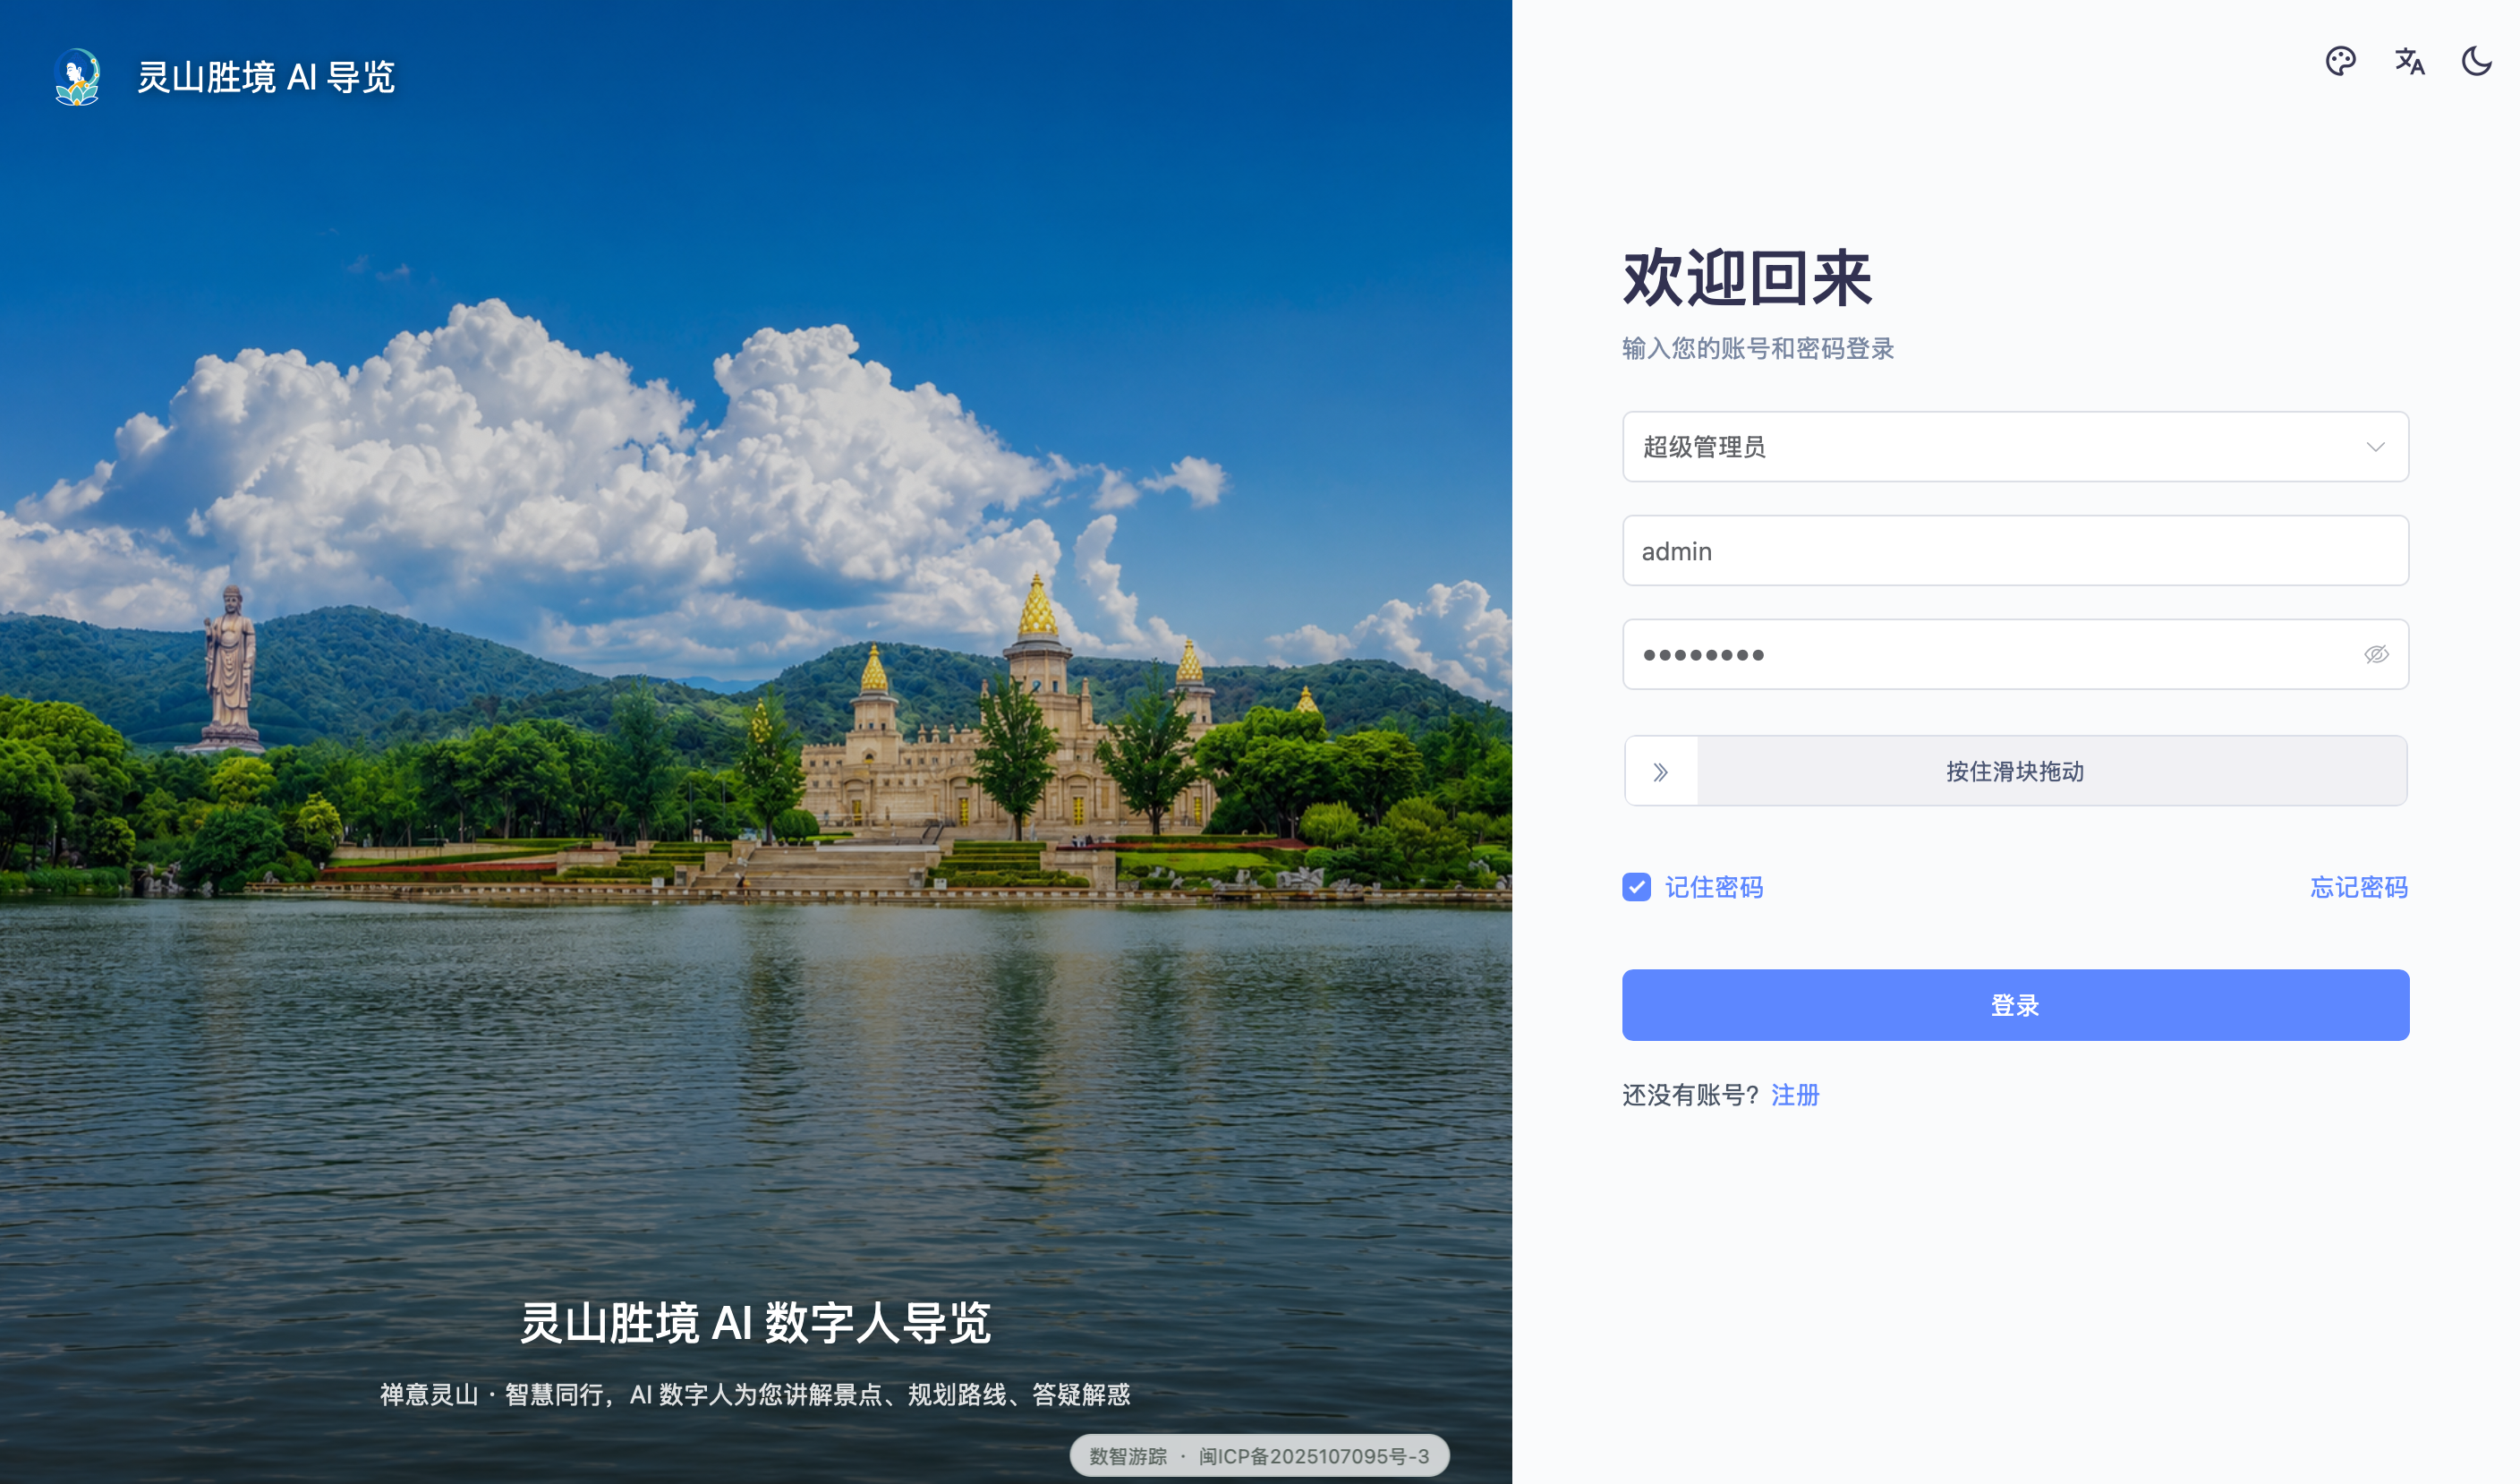
\includegraphics[width=0.95\textwidth]{assets/figures/login.png}%
  }{%
    \begin{tikzpicture}[x=1cm,y=1cm]
      \draw[rounded corners=5pt,very thick,guideTeal,fill=white] (0,0) rectangle (14.2,6.6);
      \fill[guideTeal] (0,0) rectangle (7.35,6.6);
      \node[text=white,font=\Large\bfseries] at (3.68,5.35) {数智游踪};
      \node[text=white,align=center,font=\small] at (3.68,4.60) {禅意灵山 · 智慧同行\\AI数字人景区导览与运营平台};
      \draw[white!65,rounded corners=3pt] (1.25,1.30) rectangle (6.10,3.75);
      \node[text=white,align=left,anchor=west] at (1.65,3.15) {\textbf{游客服务}\quad 问答 · 讲解 · 路线};
      \node[text=white,align=left,anchor=west] at (1.65,2.50) {\textbf{管理闭环}\quad 知识 · 数字人 · 运营};
      \node[text=white,align=left,anchor=west] at (1.65,1.85) {\textbf{可信保障}\quad 引用 · 质量 · 降级};
      \draw[rounded corners=5pt,thick,guideGray,fill=white] (8.15,0.65) rectangle (13.45,5.95);
      \node[font=\Large\bfseries,text=guideTeal] at (10.80,5.20) {管理端登录};
      \node[text=guideGray,font=\small] at (10.80,4.75) {账号验证后进入运营工作台};
      \node[anchor=west,font=\small] at (8.75,4.05) {用户名};
      \draw[rounded corners=2pt,guideGray] (8.75,3.40) rectangle (12.85,3.85);
      \node[anchor=west,text=guideGray,font=\small] at (8.95,3.62) {请输入管理员账号};
      \node[anchor=west,font=\small] at (8.75,2.95) {密码};
      \draw[rounded corners=2pt,guideGray] (8.75,2.30) rectangle (12.85,2.75);
      \node[anchor=west,text=guideGray,font=\small] at (8.95,2.52) {请输入登录密码};
      \draw[rounded corners=2pt,guideGold,fill=guideGoldLight] (8.75,1.55) rectangle (12.85,2.00);
      \node[text=guideGray,font=\small] at (10.80,1.77) {拖动滑块完成验证};
      \draw[rounded corners=2pt,guideTeal,fill=guideTeal] (8.75,0.90) rectangle (12.85,1.35);
      \node[text=white,font=\bfseries] at (10.80,1.12) {登录};
    \end{tikzpicture}%
  }
  \caption{管理端身份认证登录页面图}\label{fig:login-ui}
\end{figure}

\section{全局多语言交互}

页面右上角提供\textbf{统一语言入口}，语言选择作用于游客导览、知识库、数字人配置、运营大屏、会话反馈和系统管理等\textbf{全部路由}，而不是只替换顶部导航。切换动作同时更新\textbf{Vue i18n 活动语言与 Pinia 用户状态以}及 HTML 的\filepath{lang}属性，并通过版本化本地存储在下次访问时恢复。业务文案采用\textbf{五元组目录}维护，新增功能必须同时提供五种译文，降低遗漏单个页面或弹窗的风险。

\begin{table}[H]
  \centering
  \small
  \renewcommand{\arraystretch}{1.35}
  \caption{全局国际化语言与消息策略表}\label{tab:i18n-languages}
  \begin{tabularx}{\textwidth}{p{0.20\textwidth}p{0.13\textwidth}p{0.25\textwidth}X}
    \toprule
    界面语言 & 代码 & 基础消息来源 & 合并与回退策略 \\
    \midrule
    简体中文 & \texttt{zh} & \filepath{langs/zh.json} & 中文框架消息与完整业务消息目录 \\
    English & \texttt{en} & \filepath{langs/en.json} & 英文框架消息与完整业务消息目录，\newline 同时作为全局回退语言 \\
    韩文（Korean） & \texttt{ko} & 英文基础消息 & 合并韩文框架覆盖与韩文业务消息 \\
    繁體中文 & \texttt{zh-TW} & 简体中文基础消息 & 合并繁体框架覆盖与繁体业务消息 \\
    日本語 & \texttt{ja} & 英文基础消息 & 合并日文框架覆盖与日文业务消息 \\
    \bottomrule
  \end{tabularx}
\end{table}

\newpage
\section{游客端交互设计}

游客进入页面后由数字人播报欢迎语；可直接文字提问，也可启动语音输入。\textbf{Web端}按浏览器能力使用Web Speech API，\textbf{Android、iOS与HarmonyOS游客端}则由\filepath{uni.getRecorderManager}录音，经\filepath{uni.uploadFile}上传至\filepath{/api/voice/ask-upload}，从而复用服务端ASR--RAG--TTS链路；微信小程序在相同上传接口与权限约束下工作。问答结果同时呈现\textbf{答案、质量标签、来源和时延}，数字人按情绪标签播报。景点卡片触发约一分钟讲解，路线偏好面板采集时长、兴趣、亲子和拍照需求，结果节点可继续点击讲解。会话末尾支持\textbf{赞踩、1--5分和文字反馈}。

\begin{figure}[H]
  \centering
  \IfFileExists{assets/figures/visitor-guide.png}{%
    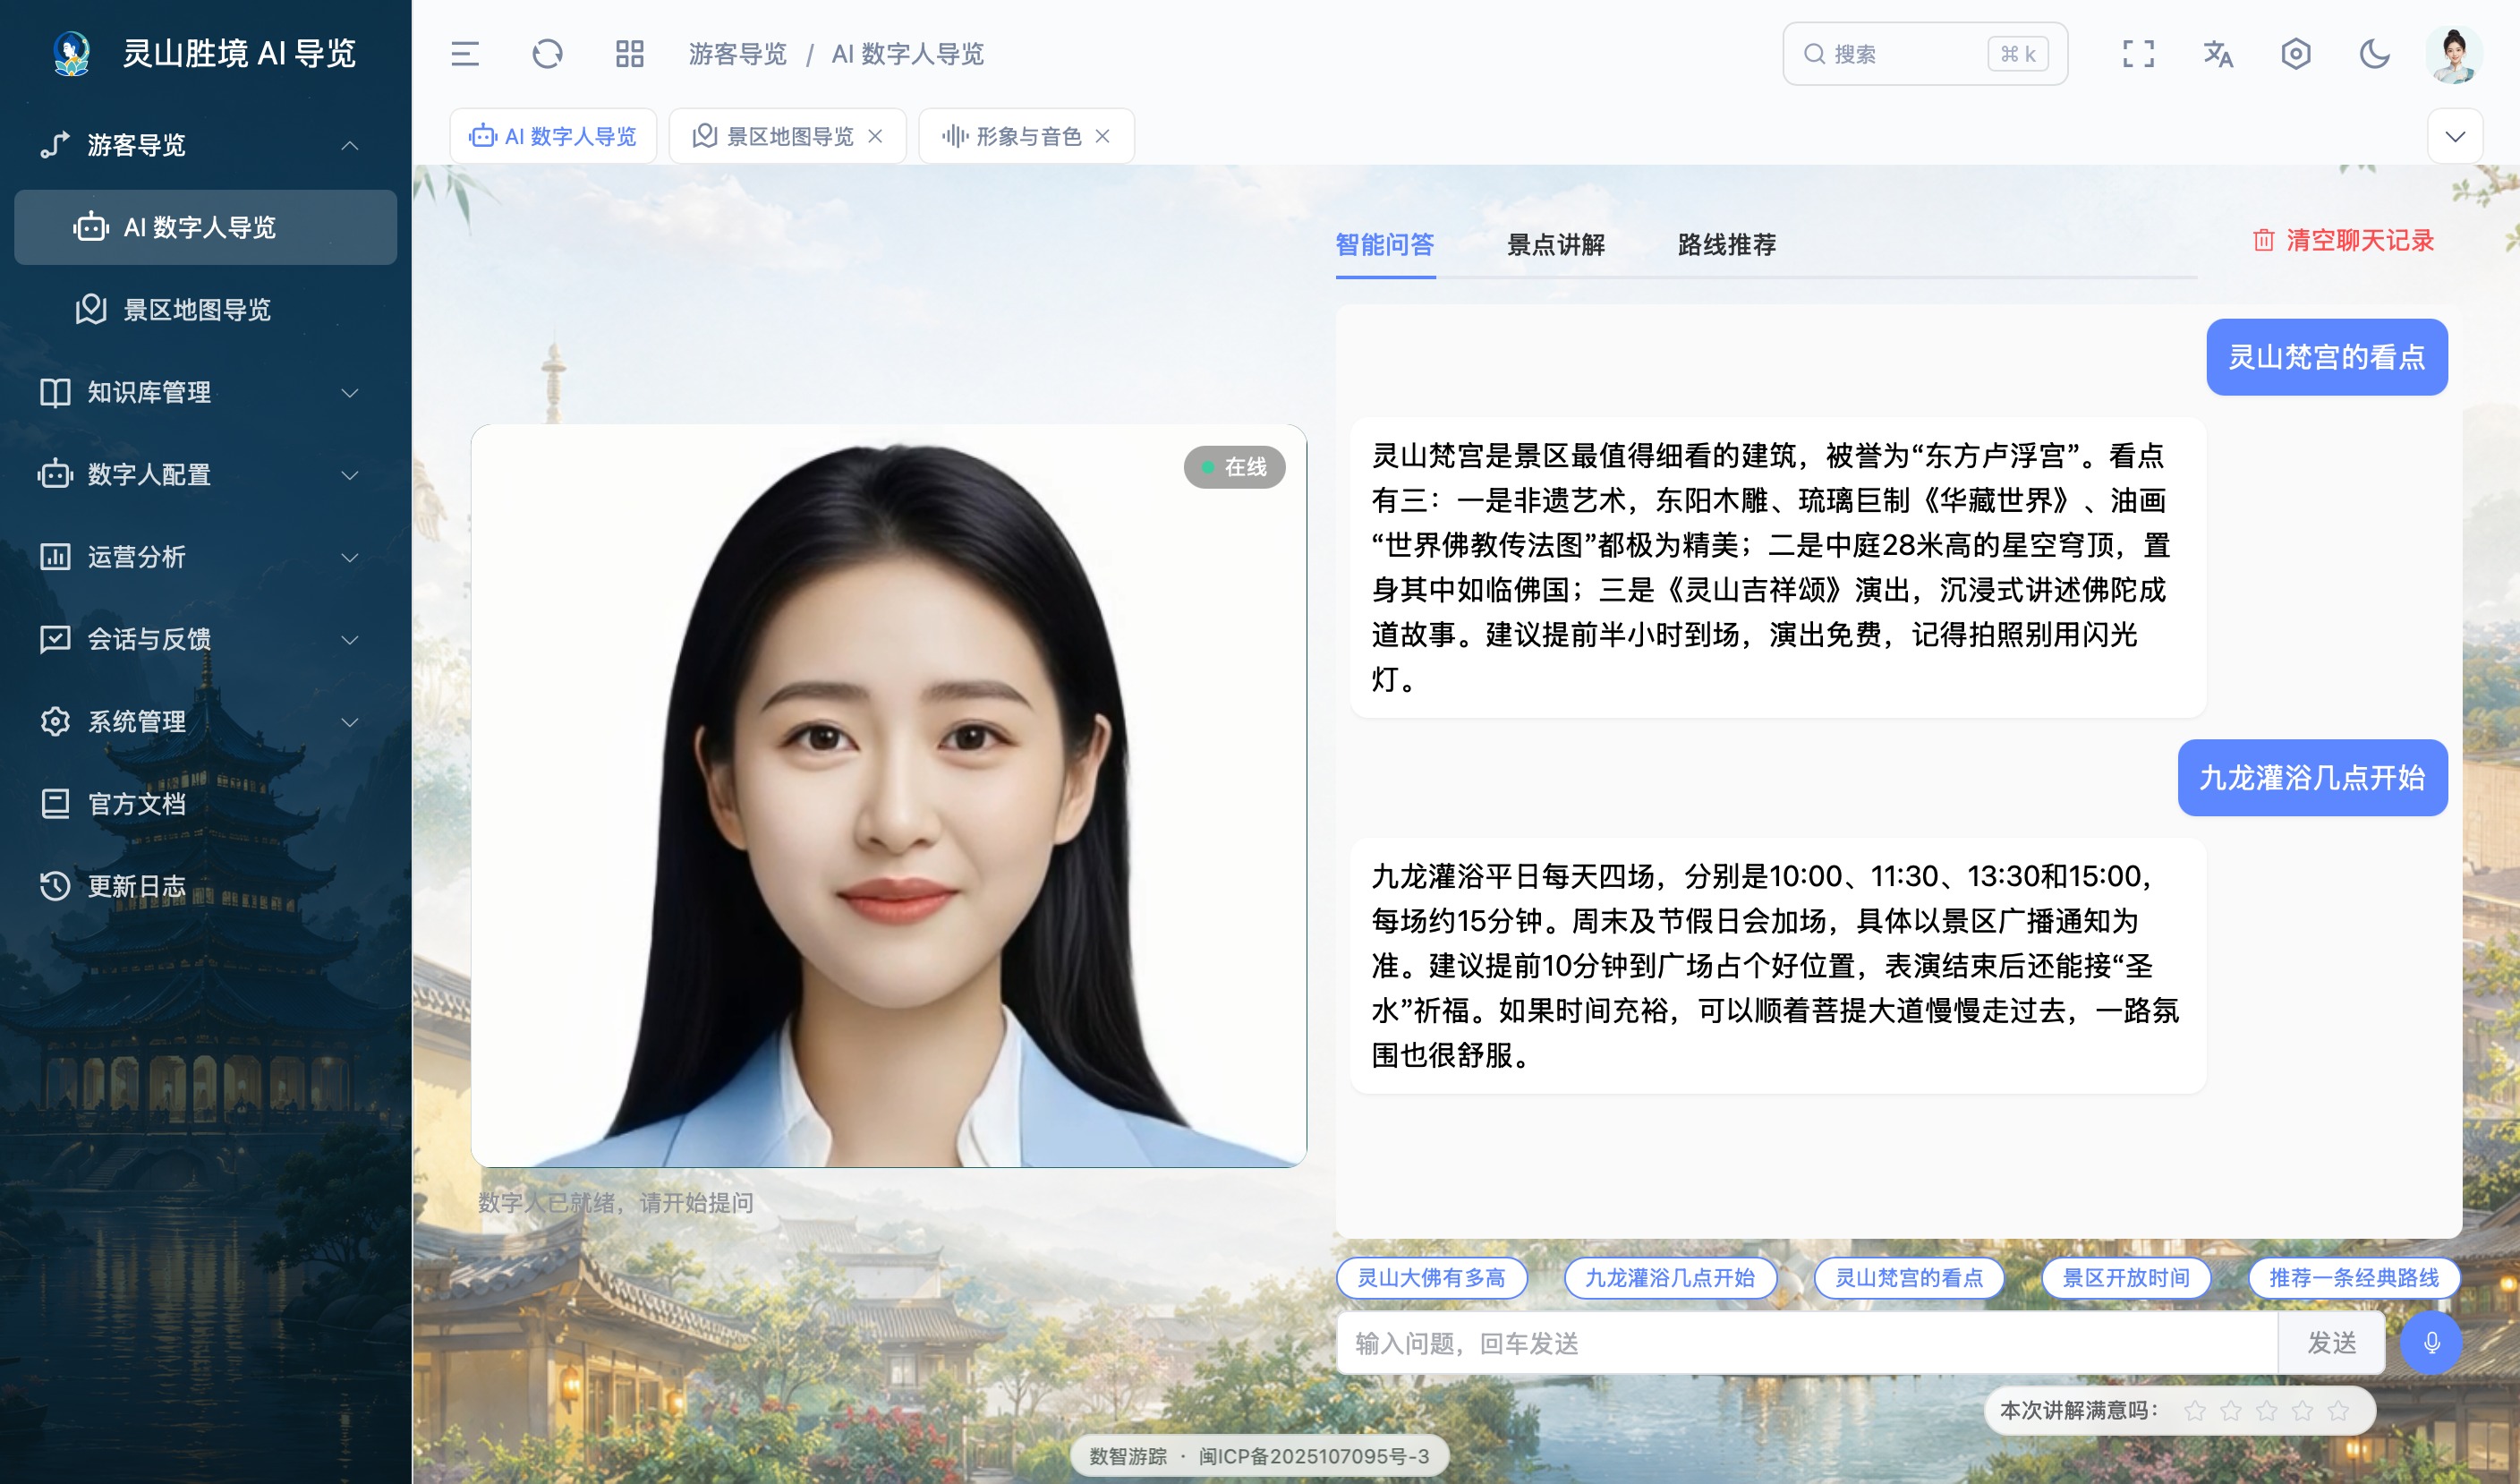
\includegraphics[width=0.95\textwidth]{assets/figures/visitor-guide.png}%
  }{%
    \begin{tikzpicture}[x=1cm,y=1cm]
      \draw[rounded corners=5pt,very thick,guideTeal,fill=guideTealLight] (0,0) rectangle (14.2,7.0);
      \fill[guideTeal] (0,6.35) rectangle (14.2,7.0);
      \node[anchor=west,text=white,font=\bfseries] at (0.35,6.68) {数智游踪 · 游客导览页截图占位};
      \draw[rounded corners=3pt,thick,guideTeal,fill=white] (0.45,0.55) rectangle (4.75,6.0);
      \node[align=center,font=\bfseries] at (2.60,5.55) {讯飞交互式数字人画面};
      \draw[dashed,guideGray] (1.10,1.50) rectangle (4.10,5.10);
      \node[align=center,text=guideGray] at (2.60,3.30) {实时视频流\\口型 / 表情 / 动作};
      \draw[rounded corners=3pt,thick,guideTeal,fill=white] (5.05,2.05) rectangle (9.45,6.0);
      \node[font=\bfseries] at (7.25,5.55) {问答与引用区};
      \draw[guideGray] (5.45,4.55) rectangle (9.05,5.20);
      \draw[guideGray] (5.45,3.55) rectangle (8.65,4.25);
      \draw[guideGray] (5.45,2.55) rectangle (9.05,3.20);
      \draw[rounded corners=3pt,thick,guideGold,fill=guideGoldLight] (9.75,2.05) rectangle (13.75,6.0);
      \node[font=\bfseries] at (11.75,5.55) {景点与路线区};
      \draw[guideGold] (10.15,4.55) rectangle (11.65,5.15);
      \draw[guideGold] (11.85,4.55) rectangle (13.35,5.15);
      \draw[guideGold] (10.15,3.55) rectangle (13.35,4.15);
      \draw[guideGold] (10.15,2.55) rectangle (13.35,3.15);
      \draw[rounded corners=3pt,thick,guideGray,fill=white] (5.05,0.55) rectangle (13.75,1.70);
      \node[text=guideGray] at (9.40,1.12) {文字/语音输入 · 快捷问题 · 满意度反馈};
    \end{tikzpicture}%
  }
  \caption{游客端AI数字人导览页面图}\label{fig:visitor-ui}
\end{figure}

\section{多端游客流程与界面适配}

游客端不是把桌面网页等比例缩小，而是以\textbf{同一业务服务、两套交互密度和按平台分支的系统能力}组织。Web与Electron桌面端保留数字人、引用、路线和地图的并列工作区，适合讲解大屏、游客中心与评审演示；uni-app x游客端使用“首页—地图—AI导游—行程—我的”五个底部入口，景点详情、账号、收藏和反馈按页面或微信分包加载。二者共享Node API、景点标识、会话结构和路线字段，但录音、定位、地图容器、WebView和文件上传分别调用浏览器或uni原生能力。

\begin{table}[H]
  \centering
  \small
  \caption{游客业务在不同终端的交互适配表}\label{tab:visitor-platform-adaptation}
  \begin{tabularx}{\textwidth}{p{0.15\textwidth}p{0.24\textwidth}p{0.25\textwidth}X}
    \toprule
    能力 & Web/桌面端 & Android/iOS/HarmonyOS & 微信小程序 \\
    \midrule
    语音输入 & Web Speech或页面录音能力，统一调用语音接口 & RecorderManager录音、uploadFile上传，服务端讯飞ASR & 同一录音上传链路，遵循小程序录音授权与包体约束 \\
    数字人 & 讯飞Web SDK在线形象，配置可切换Live2D & 受控HTTPS WebView承载讯飞形象，失败时回到本地表现与TTS & 个人主体与业务域名限制下不加载受限WebView，使用本地播报动画与讯飞云音色 \\
    地图定位 & 腾讯地图/Leaflet双路径，浏览器Geolocation & 原生\texttt{<map>}、本地手绘图与\texttt{uni.getLocation} & 原生\texttt{<map>}与GCJ-02定位，POI/算路由服务端Key能力补充 \\
    页面组织 & 多栏工作区，适合大屏和管理联动 & 五Tab移动信息架构，安全区和触控尺寸适配 & 主包五Tab，详情、账号、收藏与反馈拆为分包 \\
    \bottomrule
  \end{tabularx}
\end{table}

图\ref{fig:web-real-screens}和图\ref{fig:harmony-real-screens}均来自\textbf{当前可运行系统}，而非概念效果图。Web端展示数字人问答与景区手绘地图上的真实点位；HarmonyOS截图来自\textbf{HAP在Pura 90模拟器的安装运行结果}，覆盖首页、个人服务与AI导游主链路。Android APK与微信小程序的真实运行截图统一放在第\ref{sec:multiplatform-delivery}节，便于评审连续核对\textbf{多端交付结果}。

\begin{figure}[H]
  \centering
  \begin{minipage}[t]{0.65\textwidth}
    \centering
    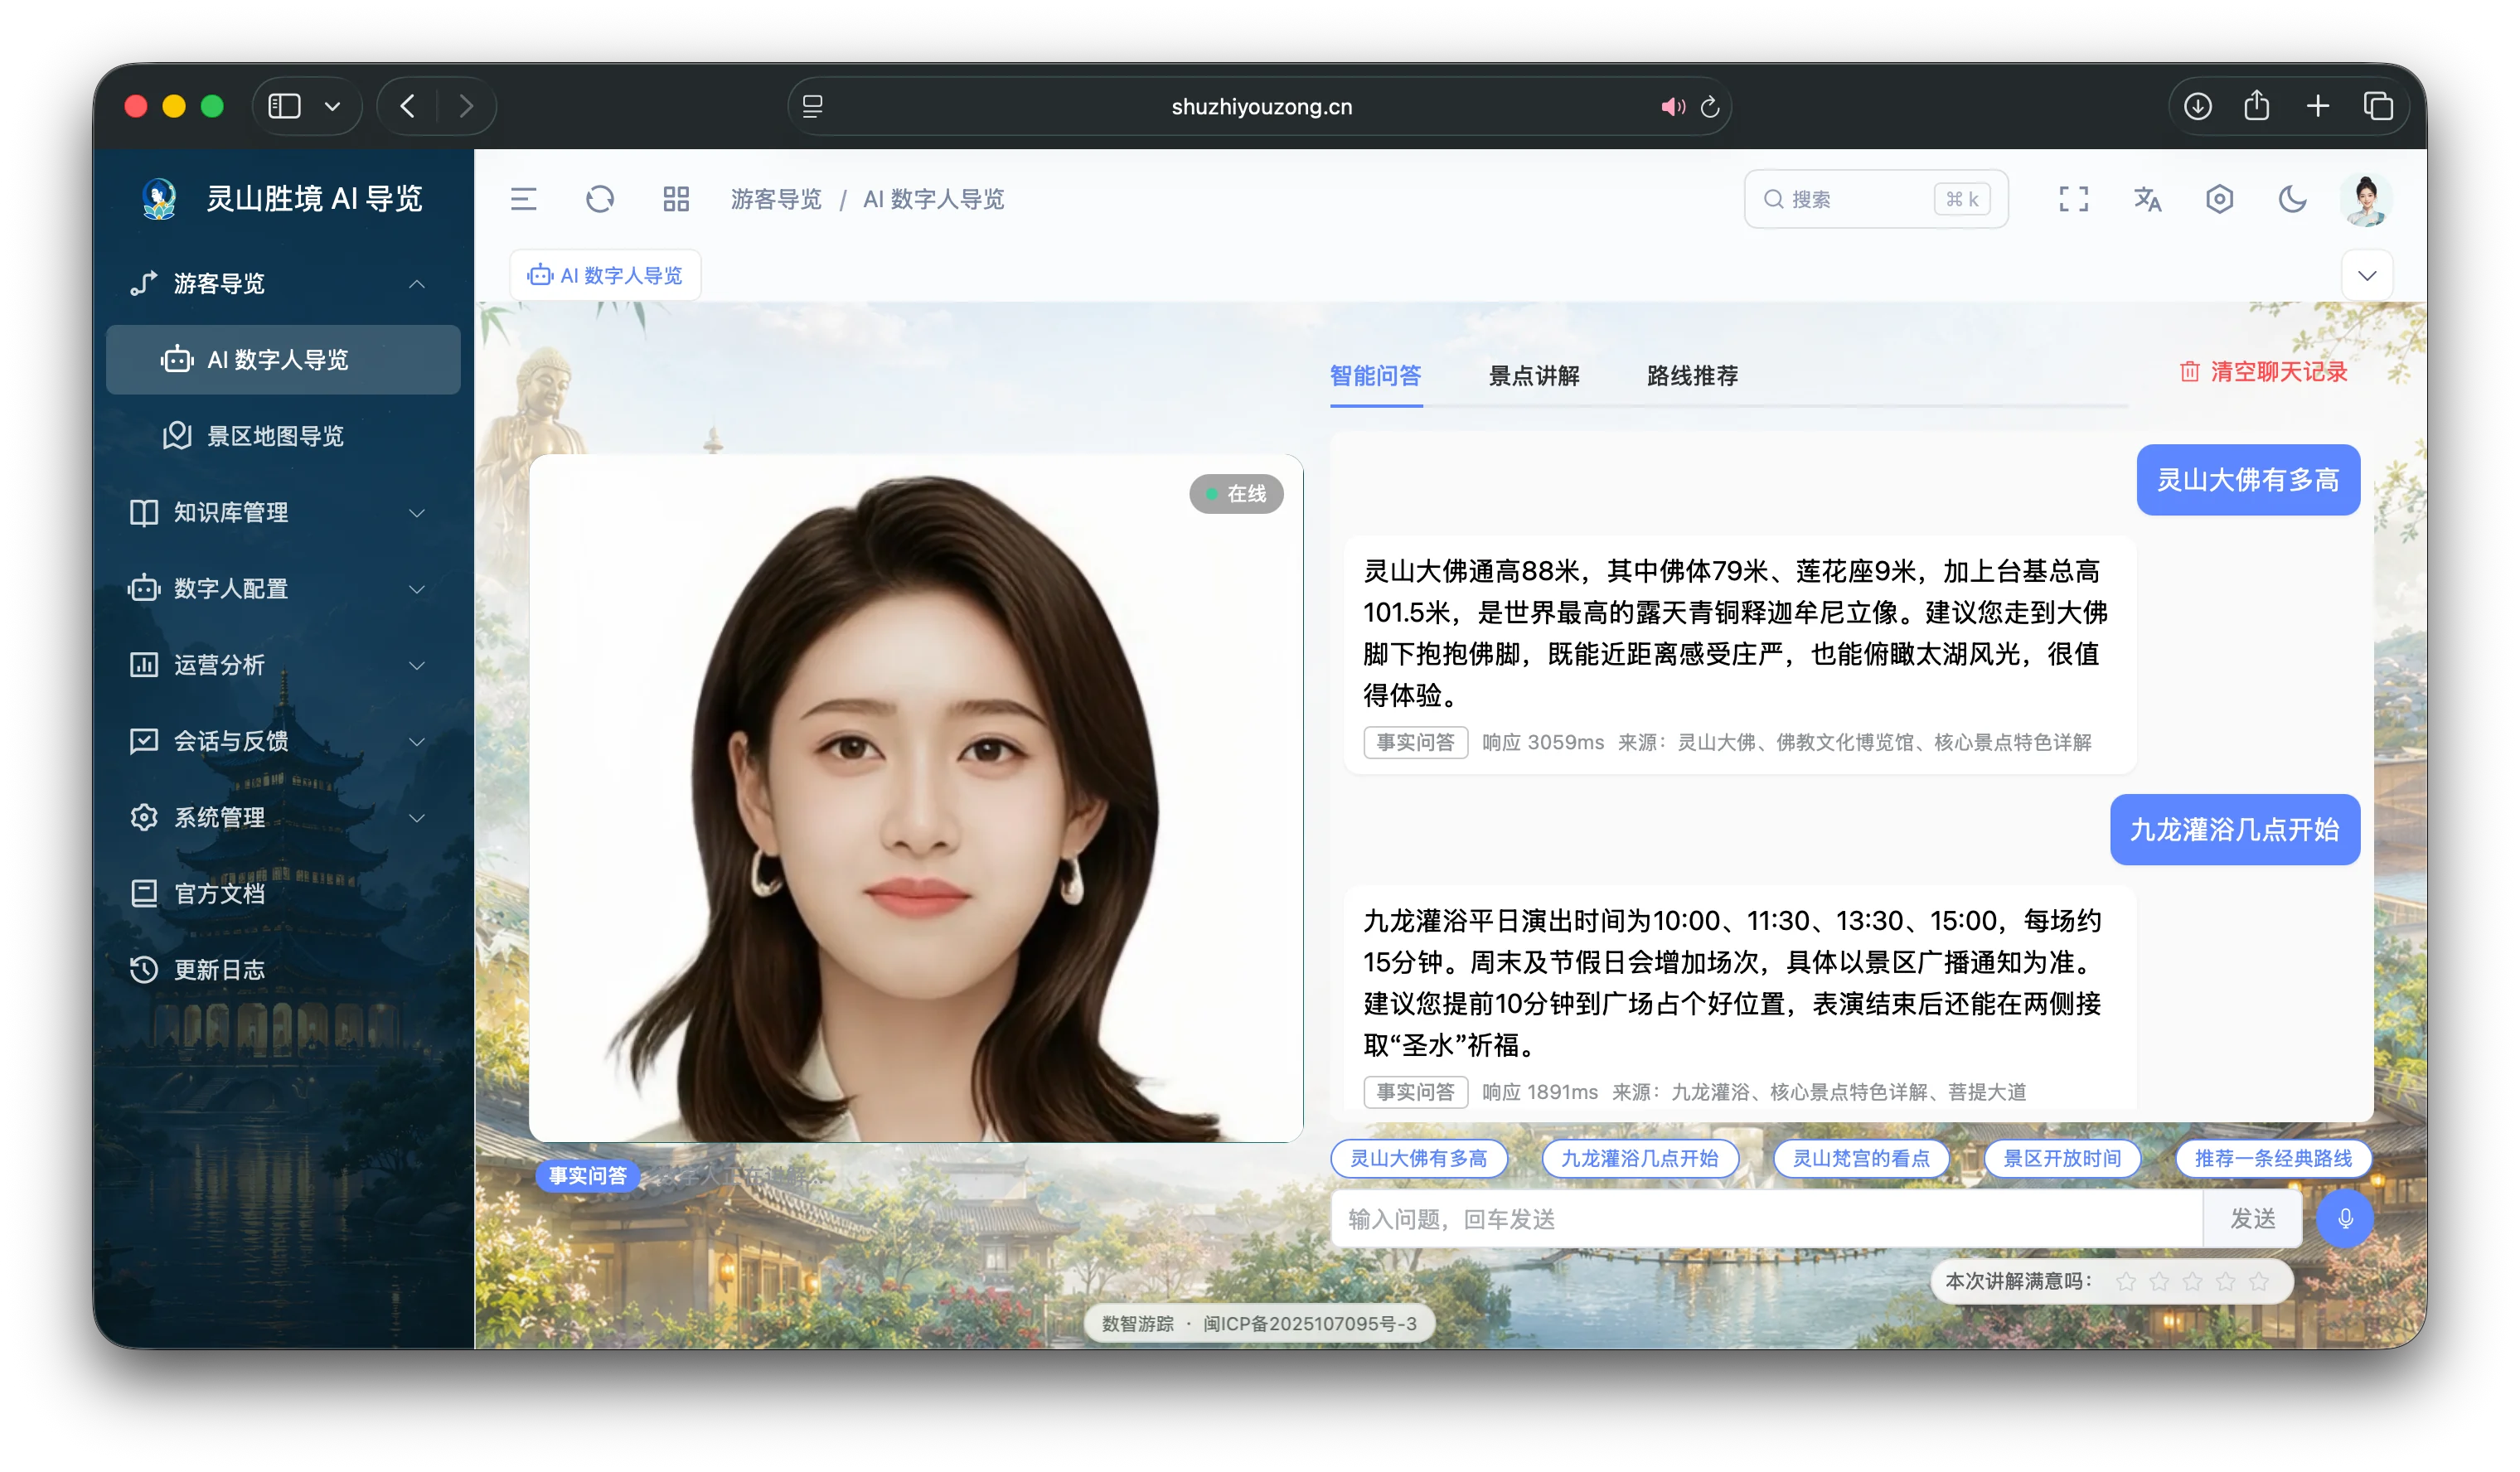
\includegraphics[width=\linewidth]{web-digital-human.png}
    \small Web在线数字人与问答界面
  \end{minipage}
  \par\medskip
  \begin{minipage}[t]{0.65\textwidth}
    \centering
    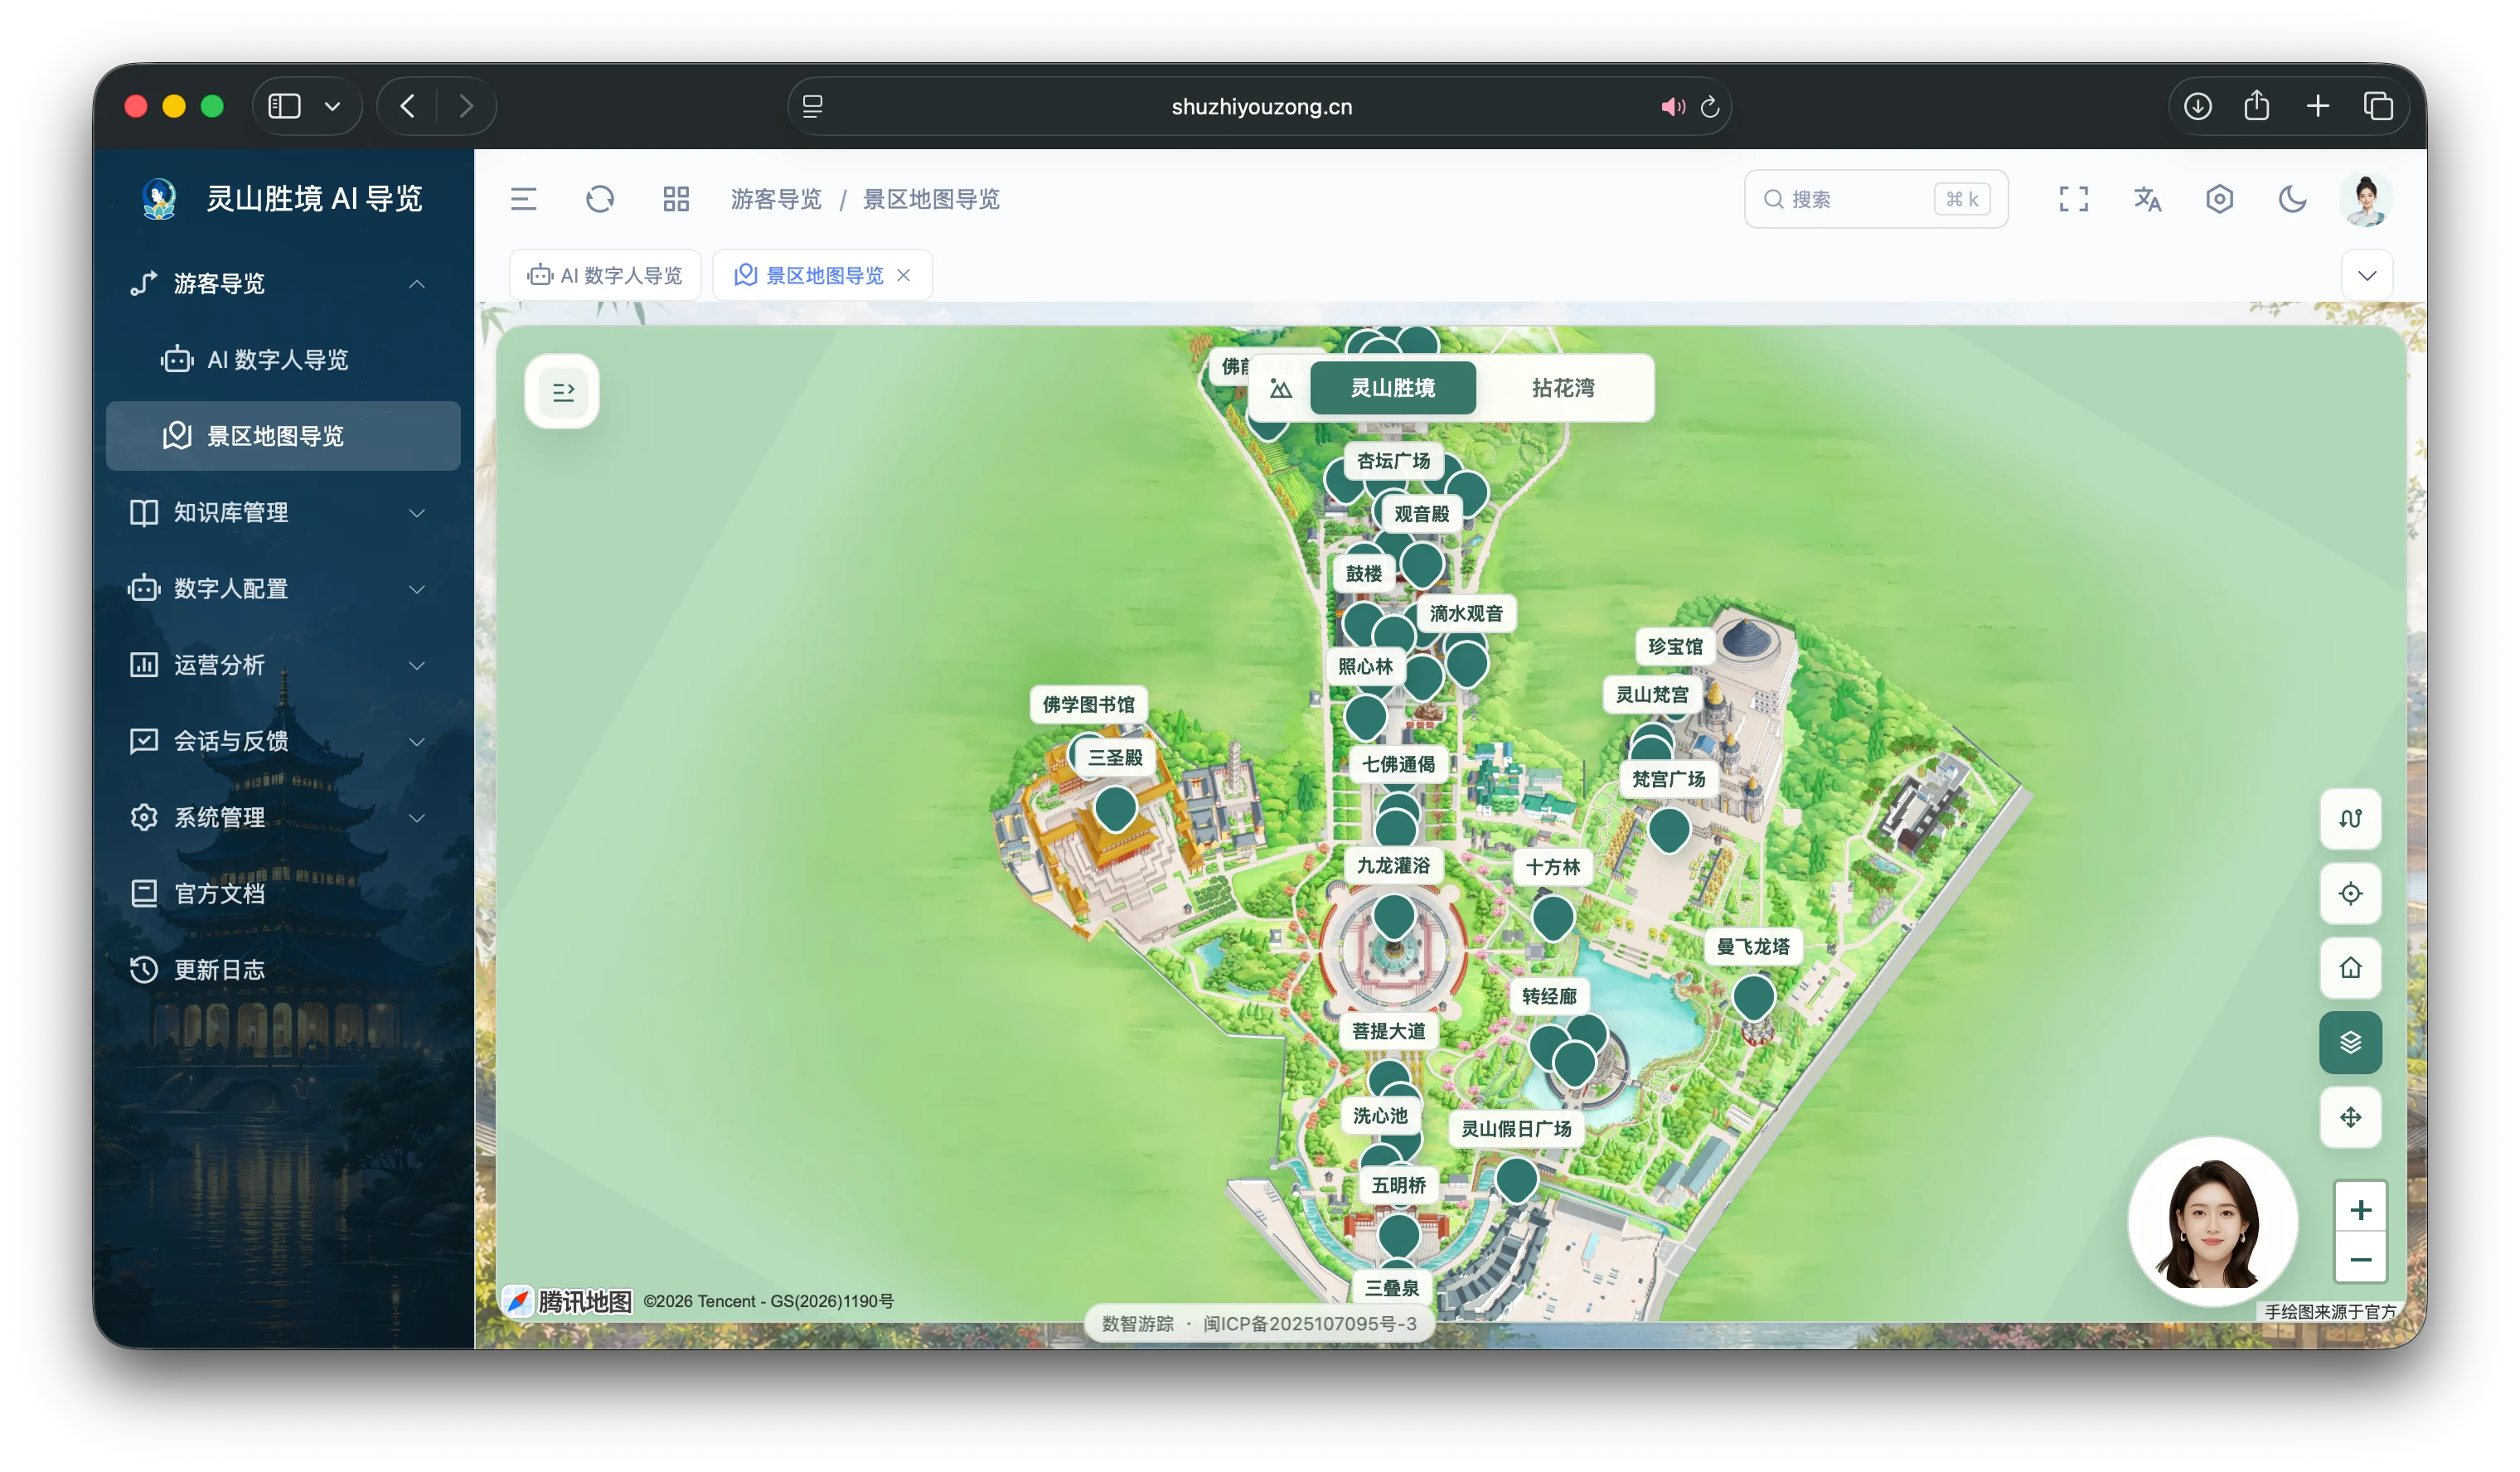
\includegraphics[width=\linewidth]{web-scenic-map.png}
    \small Web景区点位与手绘地图界面
  \end{minipage}
  \caption{Web端真实运行界面组图}\label{fig:web-real-screens}
\end{figure}

\begin{figure}[H]
  \centering
  \begin{minipage}[t]{0.30\textwidth}
    \centering
    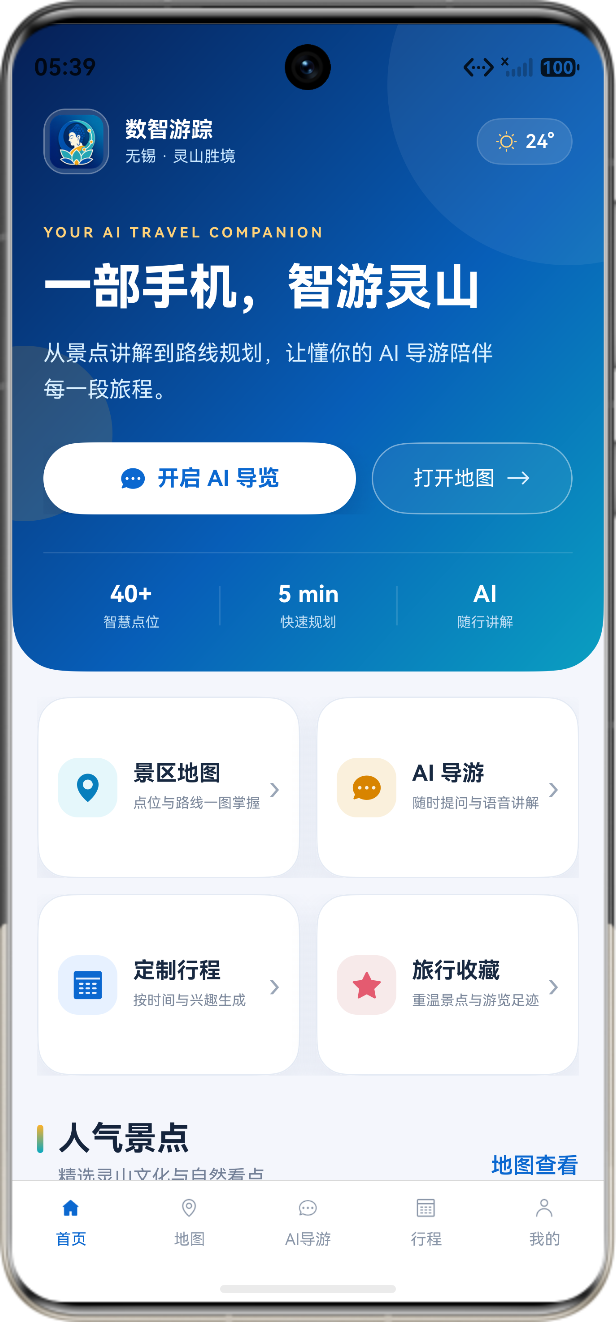
\includegraphics[width=\linewidth]{visitor-harmony-home.png}
    \small 首页与景点入口
  \end{minipage}\hfill
  \begin{minipage}[t]{0.30\textwidth}
    \centering
    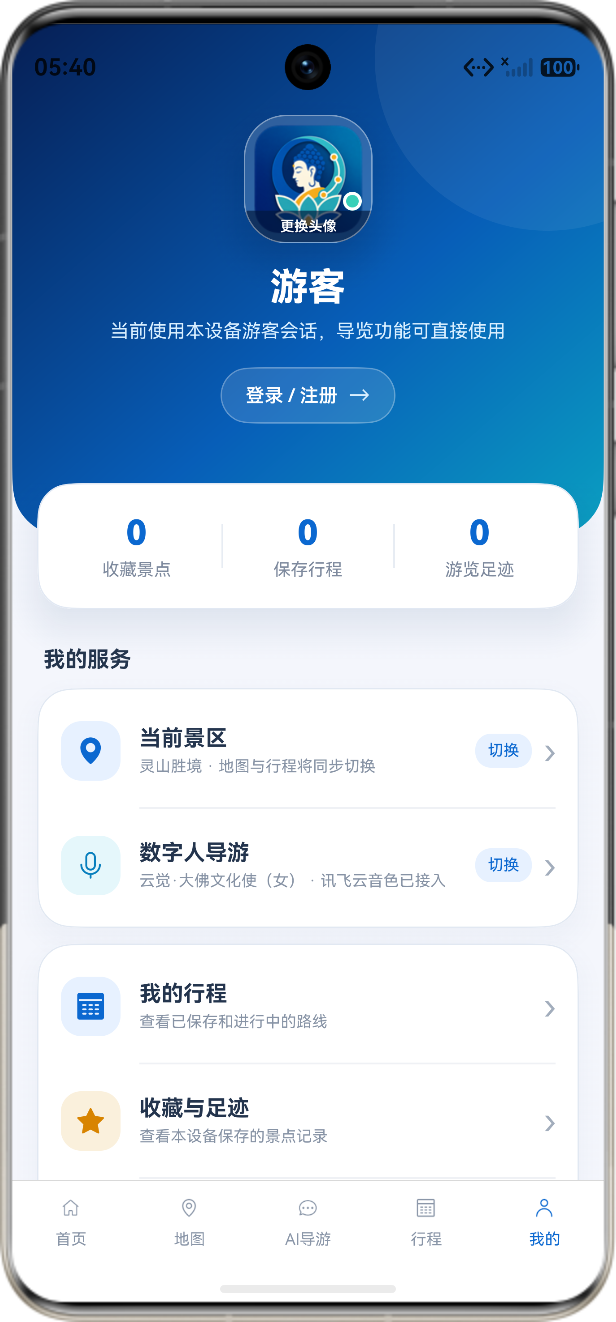
\includegraphics[width=\linewidth]{visitor-harmony-infor.png}
    \small “我的”与个人服务页面
  \end{minipage}\hfill
  \begin{minipage}[t]{0.30\textwidth}
    \centering
    
\includegraphics[width=\linewidth]{visitor-harmony-ai.png}
    \small AI导游与数字人入口
  \end{minipage}
  \caption{HarmonyOS HAP真实运行界面组图}\label{fig:harmony-real-screens}
\end{figure}

\section{多模态交互流程}

图\ref{fig:multimodal-flow}将\textbf{核心节点固定在同一水平线上}。快捷问题、云端数字人和会话记录作为扩展节点位于两侧，曲线从节点边缘出发，不穿越核心内容。

\begin{figure}[H]
  \centering
  \resizebox{0.98\textwidth}{!}{%
  \begin{tikzpicture}[x=1cm,y=1cm]
    \node[core] (m1) at (0,0) {游客输入\\语音或文本};
    \node[core] (m2) at (3.05,0) {输入标准化\\ASR/文本};
    \node[core] (m3) at (6.10,0) {可信问答\\FAQ/RAG/LLM};
    \node[coregold] (m4) at (9.15,0) {数字人表达\\TTS/口型/表情};
    \node[coregold] (m5) at (12.20,0) {反馈沉淀\\评分与会话};
    \draw[flow] (m1.east) -- (m2.west);
    \draw[flow] (m2.east) -- (m3.west);
    \draw[flowgold] (m3.east) -- (m4.west);
    \draw[flowgold] (m4.east) -- (m5.west);
    \node[side] (quick) at (0,2.0) {快捷问题\\景点卡片};
    \node[side] (sdk) at (9.15,-2.0) {讯飞WebRTC\\形象与音色};
    \node[side] (admin) at (12.20,2.0) {后台分析\\质量与趋势};
    \draw[curved] (quick.south) to[out=270,in=90] (m1.north);
    \draw[curved] (m3.south) to[out=270,in=180] (sdk.west);
    \draw[curved] (sdk.north) to[out=90,in=270] (m4.south);
    \draw[curved] (m5.north) to[out=90,in=270] (admin.south);
  \end{tikzpicture}}
  \caption{语音文本与数字人协同交互流程图}\label{fig:multimodal-flow}
\end{figure}

\newpage
\section{管理端交互设计}

管理端按业务闭环设置\textbf{六组菜单}：知识库管理、数字人配置、运营分析、会话与反馈、服务质量、系统用户。\\运营人员可在\textbf{不修改代码}的情况下维护FAQ与景点资料，并在数字人新增/编辑弹窗中展开\textbf{“选择形象”和“选择音色”}目录。选择形象会同步填入讯飞\filepath{avatarId}或Live2D \filepath{modelId}及角色名称，选择音色会写入\textbf{VCN参数}；下方表单继续支持欢迎语、语速、情绪风格、服务状态和启用开关等精细配置。

\subsection{形象模型与音色目录}

系统内置\textbf{四组讯飞云端形象和四组Live2D本地模型}，名称同时标明\textbf{性别与赛题景区元素}，便于运营人员快速判断使用场景。启用任一配置后，游客端通过\textbf{同一接口}读取并选择对应渲染引擎。

\begin{table}[H]
  \centering
  \small
  \caption{数字人快捷形象目录}\label{tab:avatar-catalog}
  \begin{tabularx}{\textwidth}{p{0.17\textwidth}p{0.27\textwidth}p{0.10\textwidth}X}
    \toprule
    引擎 & 形象名称 & 性别 & 运行标识 \\
    \midrule
    讯飞云端 & 景行·灵山迎宾使 & 男 & \texttt{cnr5dg8n2000000003} \\
    讯飞云端 & 灵悦·莲心礼宾使 & 女 & \texttt{cnrfb86h2000000004} \\
    讯飞云端 & 云觉·大佛文化使 & 女 & \texttt{cnrmkf0e2000000006} \\
    讯飞云端 & 梵音·梵宫导览使 & 女 & \texttt{cnrn9jgi2000000005} \\
    Live2D本地 & 春和·九龙灵使 & 女 & \texttt{Haru} \\
    Live2D本地 & 晴音·莲华旅伴 & 女 & \texttt{Hiyori} \\
    Live2D本地 & 知远·坛城研学使 & 男 & \texttt{Kei} \\
    Live2D本地 & 清响·禅旅伙伴 & 男 & \texttt{Hibiki} \\
    \bottomrule
  \end{tabularx}
\end{table}

音色目录既包含发言人管理资料中的\textbf{英语、台湾腔和东北话音色}，也保留项目导览链路使用的普通话男女声。界面同时展示\textbf{可读名称、语种和原始VCN}，确保配置参数与讯飞账号权限能够逐项核对。

\begin{table}[H]
  \centering
  \small
  \caption{数字人快捷音色目录}\label{tab:voice-catalog}
  \begin{tabularx}{\textwidth}{p{0.23\textwidth}p{0.22\textwidth}X}
    \toprule
    音色 & 语种/口音 & VCN参数 \\
    \midrule
    Grant & 美式英语 & \filepath{x5_EnUs_Grant_flow} \\
    台湾腔温柔男声 & 台湾普通话 & \filepath{x6_taiqiangnuannan_pro} \\
    Lila & 美式英语 & \filepath{x5_EnUs_Lila_flow} \\
    子阳 & 东北话 & \filepath{x4_ziyang_oral} \\
    聆小玥 & 普通话 & \filepath{x5_lingxiaoyue_flow} \\
    鹏飞 & 普通话 & \filepath{x4_pengfei} \\
    导览女声 & 普通话 & \filepath{x6_jingqudaolannvsheng_mini} \\
    导览男声 & 普通话 & \filepath{x6_zhantingnanjiedai_pro} \\
    \bottomrule
  \end{tabularx}
\end{table}

\begin{figure}[H]
  \centering
  \IfFileExists{web-operations-dashboard.png}{%
    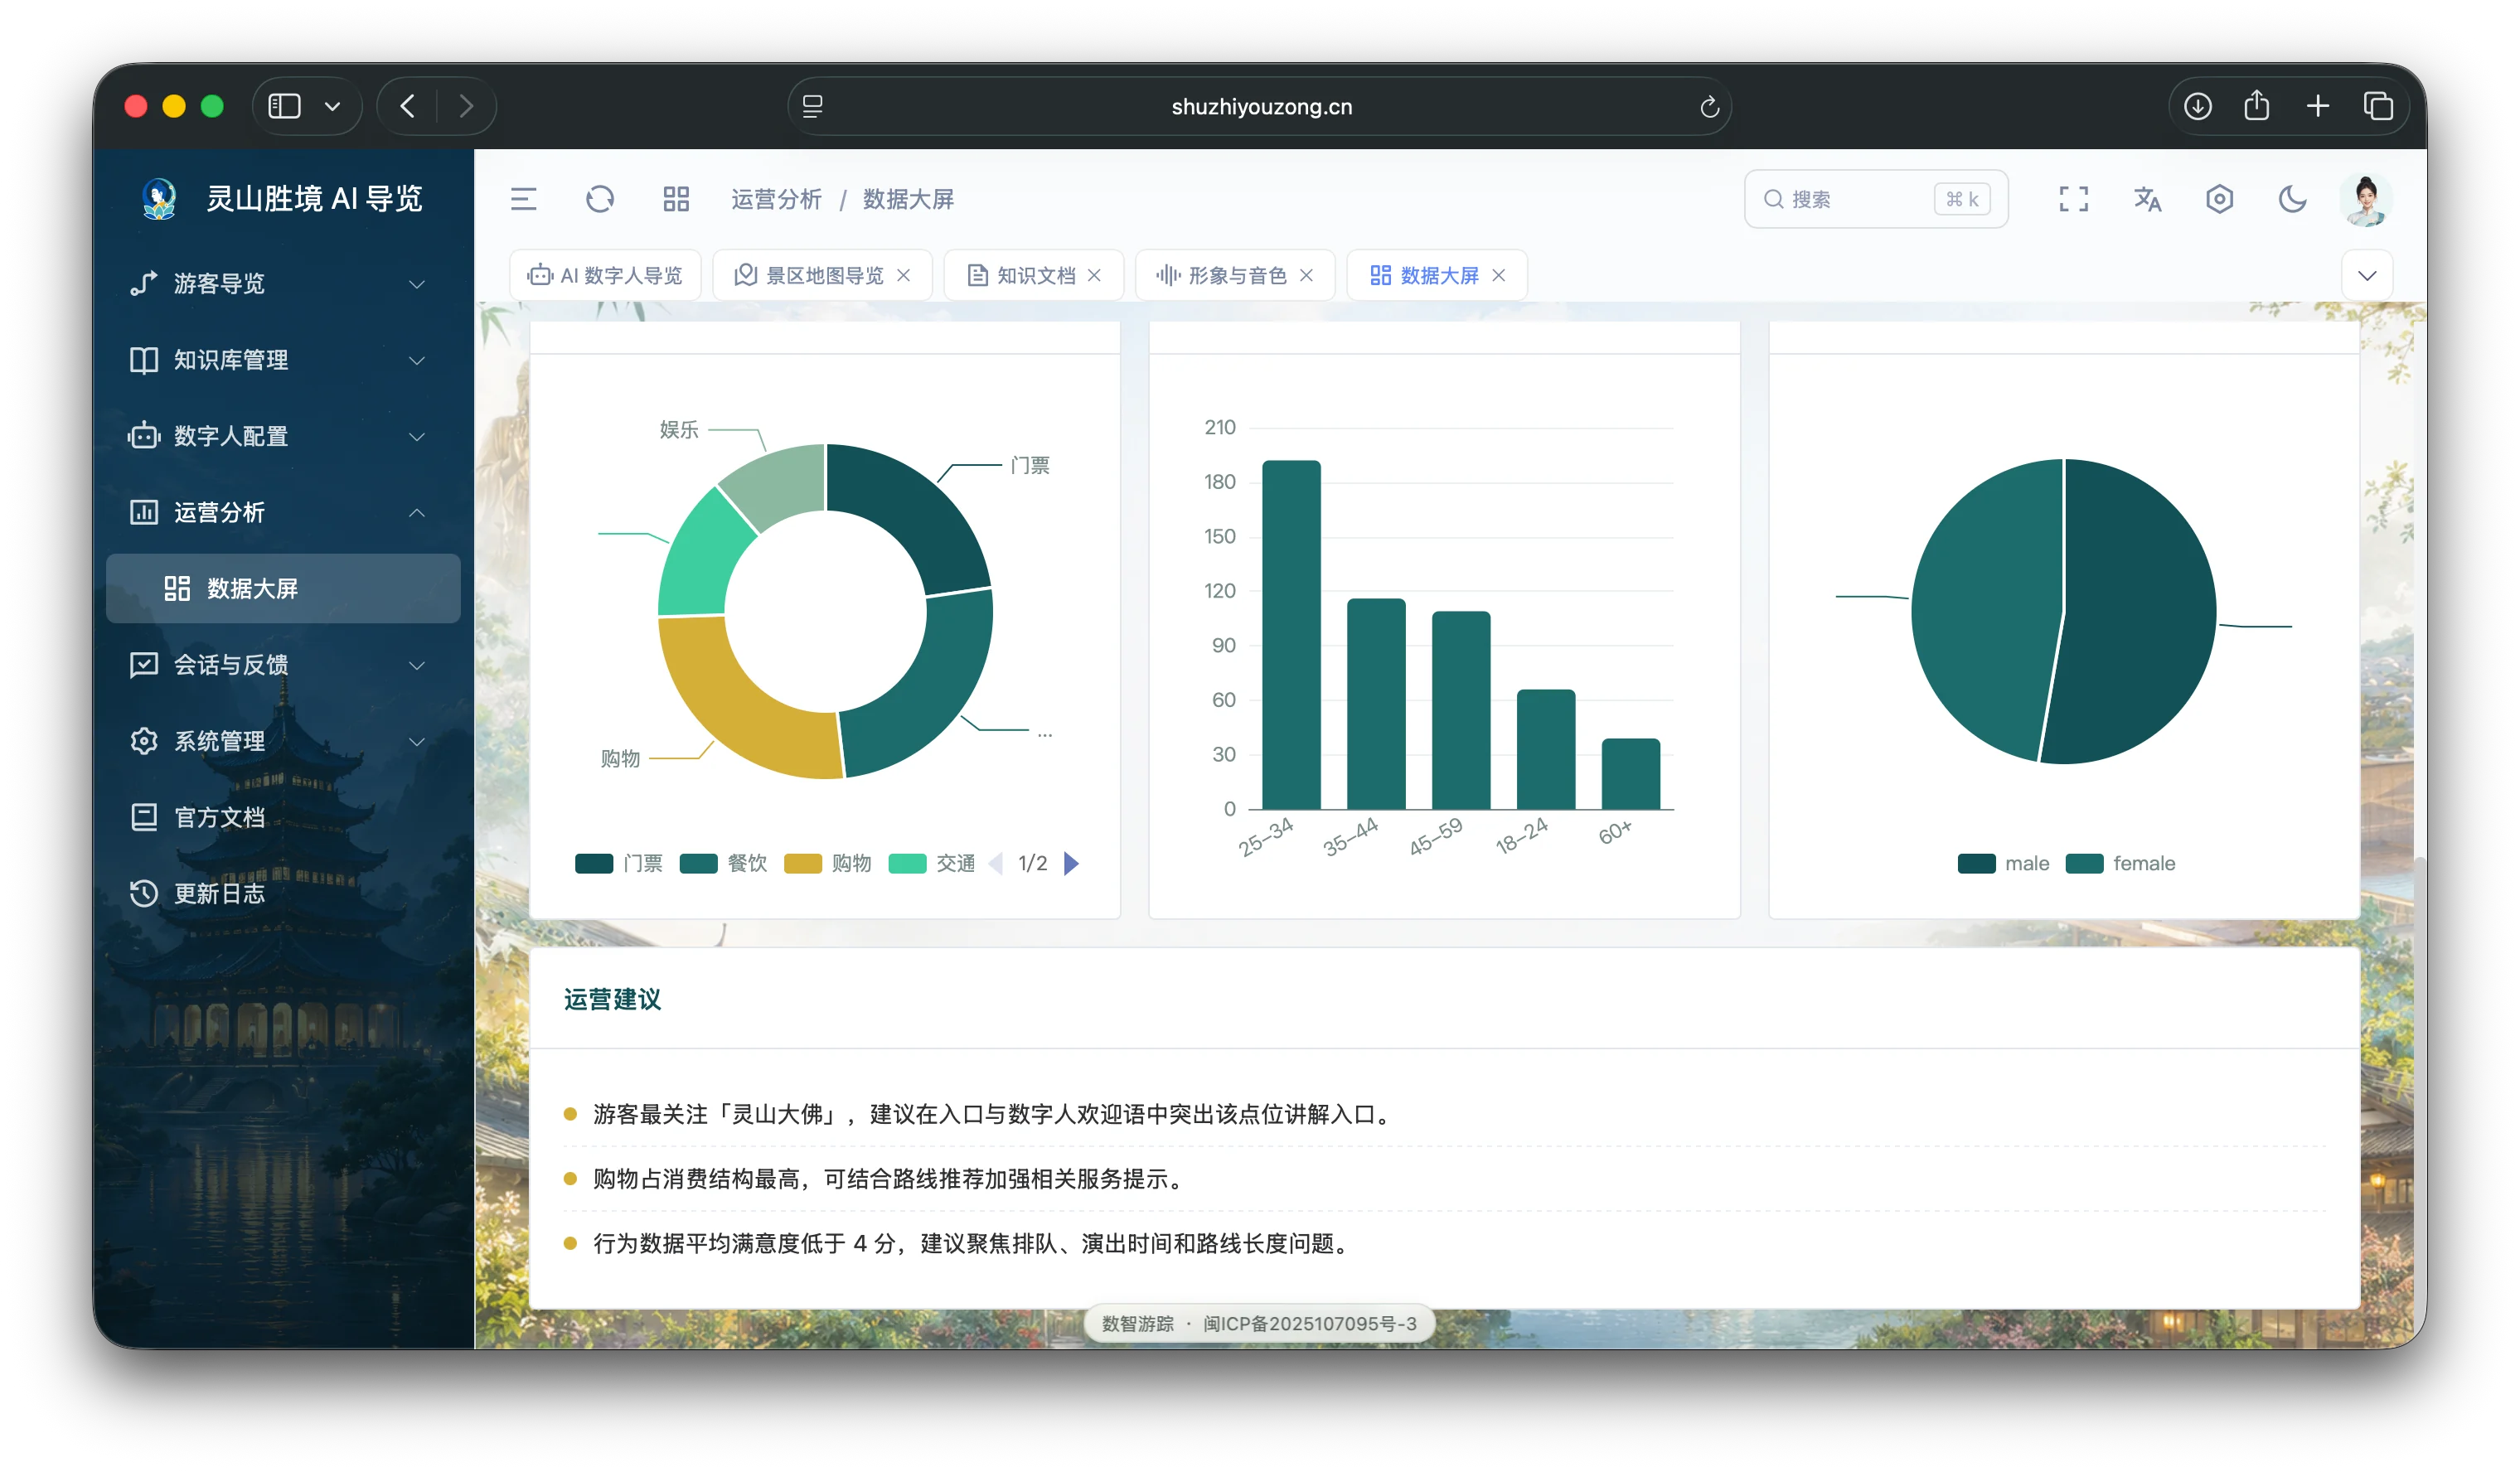
\includegraphics[width=0.86\textwidth]{web-operations-dashboard.png}%
  }{\IfFileExists{assets/figures/admin-dashboard.png}{%
    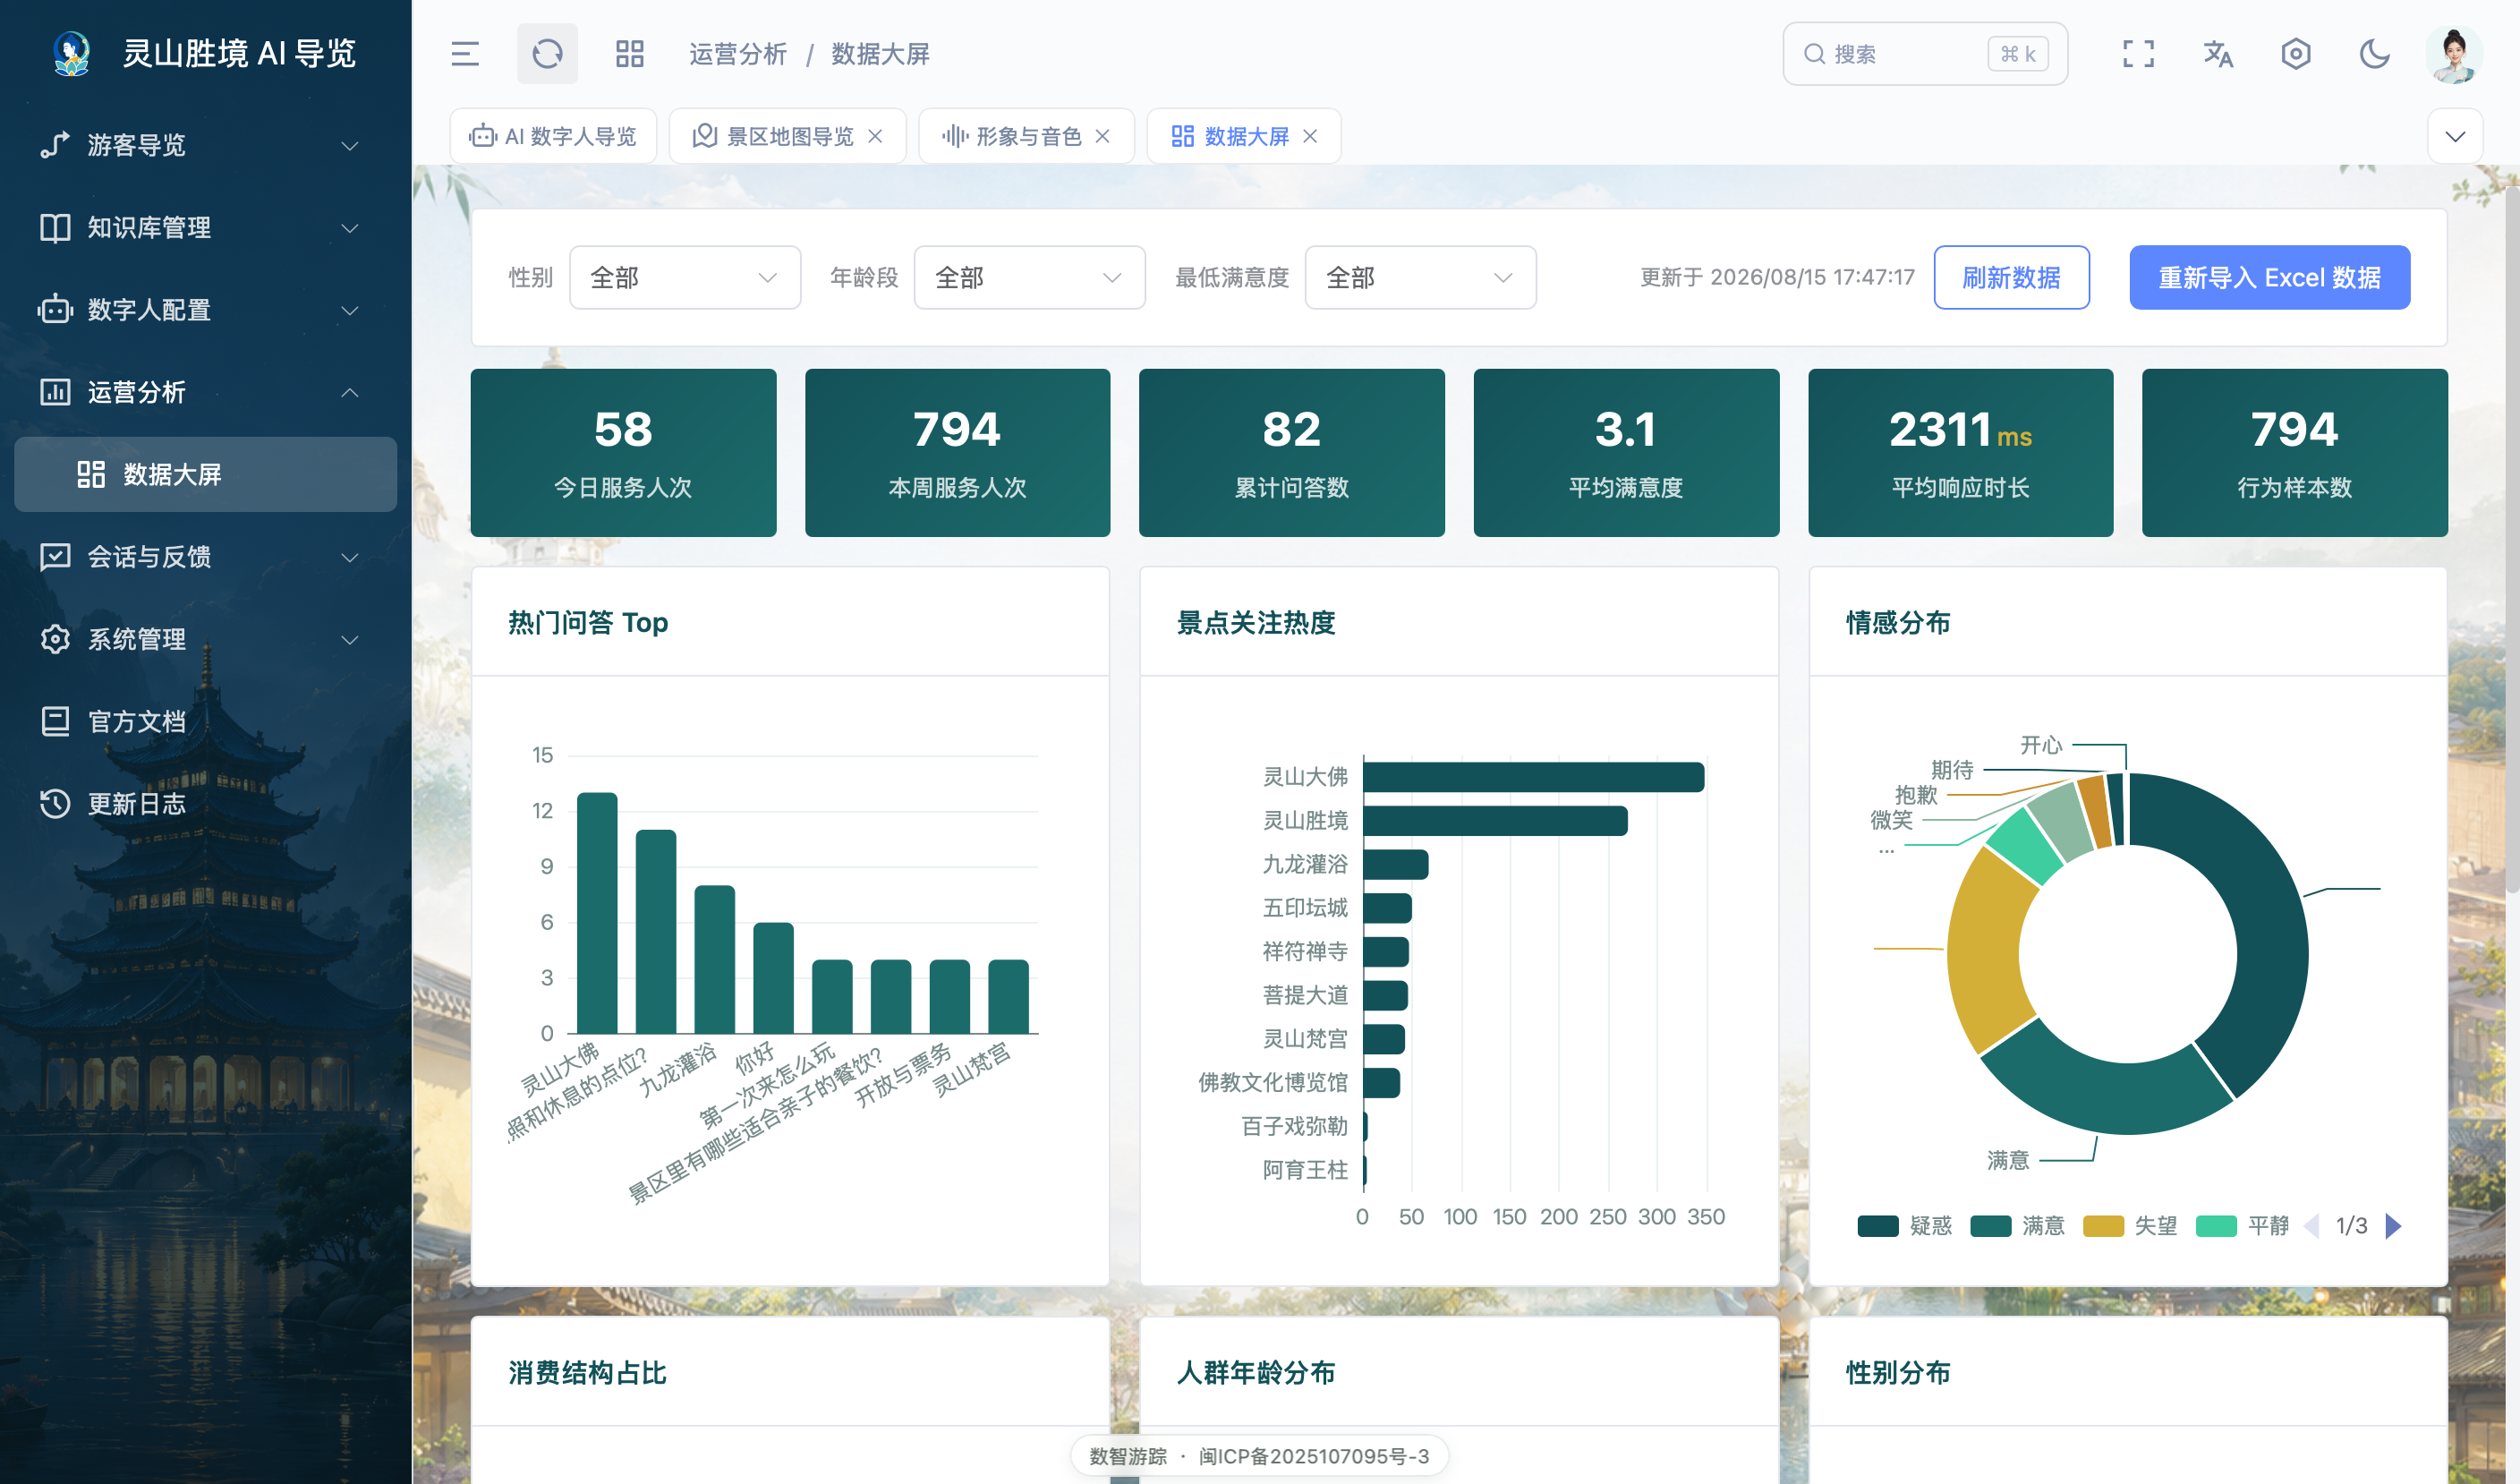
\includegraphics[width=0.86\textwidth]{assets/figures/admin-dashboard.png}%
  }{%
    \begin{tikzpicture}[x=1cm,y=1cm]
      \draw[rounded corners=5pt,very thick,guideGold,fill=guideGoldLight] (0,0) rectangle (14.2,6.9);
      \fill[guideTeal] (0,0) rectangle (2.2,6.9);
      \node[text=white,font=\bfseries,align=center] at (1.1,6.35) {数智游踪\\管理后台};
      \foreach \y/\t in {5.45/知识库管理,4.65/数字人配置,3.85/运营分析,3.05/会话与反馈,2.25/服务质量,1.45/系统管理}{
        \node[text=white,anchor=west,font=\small] at (0.38,\y) {\t};
      }
      \draw[rounded corners=3pt,fill=white,draw=guideGold] (2.55,5.25) rectangle (5.15,6.35);
      \draw[rounded corners=3pt,fill=white,draw=guideGold] (5.45,5.25) rectangle (8.05,6.35);
      \draw[rounded corners=3pt,fill=white,draw=guideGold] (8.35,5.25) rectangle (10.95,6.35);
      \draw[rounded corners=3pt,fill=white,draw=guideGold] (11.25,5.25) rectangle (13.85,6.35);
      \node at (3.85,5.80) {服务人次}; \node at (6.75,5.80) {满意度};
      \node at (9.65,5.80) {平均时延}; \node at (12.55,5.80) {问答总量};
      \draw[rounded corners=3pt,fill=white,draw=guideGold] (2.55,2.95) rectangle (8.05,4.90);
      \draw[rounded corners=3pt,fill=white,draw=guideGold] (8.35,2.95) rectangle (13.85,4.90);
      \draw[guideTeal,very thick] (3.05,3.35) -- (4.10,4.05) -- (5.15,3.75) -- (6.20,4.45) -- (7.55,4.15);
      \node[text=guideGray] at (5.30,3.10) {趋势与景点热度};
      \draw[fill=guideTealLight,draw=guideTeal] (8.90,3.35) rectangle (9.55,4.30);
      \draw[fill=guideGoldLight,draw=guideGold] (9.90,3.35) rectangle (10.55,4.60);
      \draw[fill=guideTealLight,draw=guideTeal] (10.90,3.35) rectangle (11.55,4.05);
      \draw[fill=guideGoldLight,draw=guideGold] (11.90,3.35) rectangle (12.55,4.40);
      \draw[rounded corners=3pt,fill=white,draw=guideGold] (2.55,0.55) rectangle (13.85,2.55);
      \node[text=guideGray] at (8.20,1.55) {消费结构 · 游客画像 · 热门问题 · 运营建议};
    \end{tikzpicture}%
  }}
  \caption{管理端运营分析大屏页面图}\label{fig:admin-ui}
\end{figure}

图\ref{fig:admin-ui}把服务人次、满意度、平均时延、问答总量、景点热度、游客画像和运营建议放在同一观察面板中。它与上文的知识库、数字人配置和会话反馈入口形成\textbf{“配置—服务—观察—修正”}闭环，评审时可以沿同一页面理解管理端如何把游客数据转化为内容维护动作。

\newpage\chapter{核心技术与算法设计}

\section{全局五语言i18n架构}

系统以\textbf{单一Vue I18n实例}承载简体中文、英文、韩文、繁体中文和日文。与仅替换框架菜单的局部国际化不同，系统把\textbf{景区业务文案}单独整理为\filepath{app.*}命名空间，并与原有框架词典合并，因此游客问答、景点与路线、数字人状态、管理表单、运营指标、会话反馈和提示弹窗均从同一活动语言解析。

业务词典按\filepath{zh}、\filepath{en}、\filepath{ko}、\filepath{zh-TW}、\filepath{ja}五个固定位置声明，每个键在构建阶段必须具有\textbf{完整五元组}。\\\filepath{LanguageEnum}提供\textbf{唯一语言代码集合}。简体中文与英文使用完整基础JSON，韩文和日文以英文框架消息为基底，繁体中文以简体中文为基底，再叠加\filepath{framework-messages.ts}的框架覆盖与\filepath{app-messages.ts}的完整业务译文。最终\textbf{未命中项回退英文}，避免渲染空白。

\begin{table}[H]
  \centering
  \small
  \renewcommand{\arraystretch}{1.35}
  \caption{国际化分层实现表}\label{tab:i18n-architecture}
  \begin{tabularx}{\textwidth}{p{0.24\textwidth}p{0.31\textwidth}X}
    \toprule
    层次 & 关键实现 & 技术作用 \\
    \midrule
    语言模型 & \filepath{LanguageEnum}、\filepath{languageOptions} & 统一五种Locale代码与界面选择顺序 \\
    基础框架词典 & \filepath{langs/zh.json}、\filepath{langs/en.json} & 提供布局、设置、表格等完整基础消息 \\
    框架覆盖词典 & \filepath{framework-messages.ts} & 补齐韩文、繁体中文、日文的框架级消息 \\
    景区业务词典 & \filepath{app-messages.ts} & 以五元组维护全部游客端与管理端业务文\newline 案 \\
    切换与持久化 & 顶部语言入口、\newline\filepath{userStore.language} & 同步Locale、页面标题、HTML语言属性与本地偏好 \\
    \bottomrule
  \end{tabularx}
\end{table}

用户选择语言后，顶部栏\textbf{同时更新全局语言状态}，包括\filepath{locale}、Pinia语言状态和\filepath{document.documentElement.lang}，\\并刷新路由标题、菜单、面包屑和工作标签。应用启动时先读取\textbf{版本化用户存储}，再兼容旧系统存储，均无记录时使用简体中文。游客端的浏览器语音识别与管理端欢迎语试听还会把Locale映射为\filepath{zh-CN}、\filepath{en-US}、\filepath{ko-KR}、\filepath{zh-TW}或\filepath{ja-JP}。

需要明确的是，当前国际化对象是\textbf{界面文案、路由元信息和浏览器语音Locale}；景点资料、历史会话及RAG/LLM生成内容保持其数据原始语言，\textbf{不在前端运行时执行机器翻译}。

\noindent\textit{源码位置：}
\begin{itemize}
  \item \filepath{web/src/locales/index.ts}
  \item \filepath{web/src/locales/app-messages.ts}
  \item \filepath{web/src/components/core/layouts/art-header-bar/index.vue}
\end{itemize}

\newpage
\lstinputlisting[style=projectcode,firstnumber=1,
  caption={五语言词典合并与全局切换核心代码},label={lst:i18n}]
  {assets/code/i18n-core.ts}

\newpage
\section{本地知识库与RAG问答}

Transformer为当前主流大模型提供了基于注意力的序列建模基础\upcite{vaswani2017attention}。RAG进一步将参数化生成模型与外部非参数知识结合，使\textbf{知识更新、证据追踪和事实约束}成为可能\upcite{lewis2020rag}。本项目采用适合比赛资料规模的\textbf{本地混合检索}：景点实体、标题、关键词、正文、同义扩展、意图和查询覆盖度共同计分；检索结果经重排后\textbf{最多选择3条引用}进入答案。

\begin{figure}[H]
  \centering
  \resizebox{0.75\textwidth}{!}{%
  \begin{tikzpicture}[x=1cm,y=1cm]
    \node[core] (r1) at (0,0) {问题输入\\上下文补全};
    \node[core] (r2) at (2.75,0) {安全护栏\\范围与敏感};
    \node[core] (r3) at (5.50,0) {混合检索\\实体/词项/意图};
    \node[core] (r4) at (8.25,0) {规则重排\\Top-K证据};
    \node[coregold] (r5) at (11.00,0) {大模型生成\\有据回答};
    \node[coregold] (r6) at (13.75,0) {响应封装\\引用/标签/耗时};
    \draw[flow] (r1.east) -- (r2.west);
    \draw[flow] (r2.east) -- (r3.west);
    \draw[flow] (r3.east) -- (r4.west);
    \draw[flowgold] (r4.east) -- (r5.west);
    \draw[flowgold] (r5.east) -- (r6.west);
    \node[side] (faq) at (2.75,2.05) {FAQ缓存\\高频快速路径};
    \node[side] (kb) at (6.85,-2.05) {本地知识库\\22景点/44分块};
    \node[side] (reject) at (11.00,2.05) {拒答策略\\越界/无资料};
    \draw[curved] (r1.north) to[out=90,in=180] (faq.west);
    \draw[curved] (faq.north) .. controls (2.75,4.25) and (15.25,4.25) .. (r6.east);
    \draw[curved] (kb.north west) to[out=135,in=270] (r3.south);
    \draw[curved] (r4.south) to[out=270,in=45] (kb.north east);
    \draw[curved] (r2.north) .. controls (4.50,1.20) and (8.80,1.20) .. (reject.west);
    \draw[curved] (reject.south) to[out=270,in=90] (r5.north);
  \end{tikzpicture}}
  \caption{本地知识库RAG可信问答流程图}\label{fig:rag-flow}
\end{figure}

\begin{algorithm}[H]
  \caption{混合检索与有据生成算法}\label{alg:rag}
  \begin{algorithmic}[1]
    \Require 问题$q$、会话历史$H$、知识分块集合$D$、返回数量$k$
    \Ensure 答案$a$、引用集合$C$、质量与情绪标签
    \State $q' \gets \Call{ResolveFollowUp}{q,H}$ \Comment{补全多轮指代}
    \If{$q'$命中敏感规则或超出景区范围}
      \State \Return 拒答结果及引导语 \Comment{先执行安全边界}
    \EndIf
    \If{FAQ缓存命中$q'$}
      \State \Return 缓存答案与零检索耗时 \Comment{高频问题快速返回}
    \EndIf
    \State $T \gets \Call{TokenizeAndExpand}{q'}$
    \State $I \gets \Call{DetectIntent}{q',T}$，$S \gets \Call{MatchSpot}{q',T}$
    \State $(w_s,w_t,w_i,w_c) \gets \Call{Calibrate}{TestSet}$ \Comment{权重由测试集校准}
    \ForAll{$d \in D$}
      \State $score[d] \gets w_sS+w_tT+w_iI+w_c\Call{Coverage}{q',d}$
    \EndFor
    \State $C \gets \Call{RerankAndTopK}{D,score,k}$ \Comment{实体与开放时间保持强约束}
    \Statex \Comment{多景区大规模语料可融合DPR稠密召回\upcite{karpukhin2020dpr}}
    \If{$C$为空或相关性低于阈值}
      \State \Return 资料未覆盖结果 \Comment{无证据不生成事实}
    \EndIf
    \State $a \gets \Call{LLMGenerate}{q',H,C}$ \Comment{只注入已选证据}
    \State \Return $a,C,\Call{Label}{q',a}$
  \end{algorithmic}
\end{algorithm}

\newpage
\noindent\textit{源码位置：}\filepath{server/src/services/retrieval.mjs}。
\lstinputlisting[style=projectcode,firstnumber=210,
  caption={景点实体与词项混合评分核心代码},label={lst:retrieval}]
  {assets/code/retrieval-score.mjs}

\newpage
\noindent\textit{源码位置：}\filepath{server/src/services/chat.mjs}。
\lstinputlisting[style=projectcode,firstnumber=195,
  caption={护栏检索与问答场景编排核心代码},label={lst:chat}]
  {assets/code/chat-orchestration.mjs}

\section{个性化路线推荐}

路线模块将景区节点、模板路线和游客偏好统一为\textbf{可解释的规则评分}。\textbf{时长匹配}形成基础分，历史文化、佛教、自然、拍照、亲子、演艺和轻松步行等标签形成增益；体力限制会降低登高节点权重。得分最高的模板再经过“30分钟压缩”“避台阶”和“冲突兴趣折中”等\textbf{自适应步骤}。

\begin{figure}[H]
  \centering
  \resizebox{0.96\textwidth}{!}{%
  \begin{tikzpicture}[x=1cm,y=1cm]
    \node[core] (t1) at (0,0) {偏好采集\\时长/兴趣/体力};
    \node[core] (t2) at (3.05,0) {偏好归一\\布尔与标签};
    \node[core] (t3) at (6.10,0) {模板评分\\时长+主题};
    \node[coregold] (t4) at (9.15,0) {路线自适应\\压缩/避阶};
    \node[coregold] (t5) at (12.20,0) {结果解释\\节点/理由/备选};
    \draw[flow] (t1.east) -- (t2.west);
    \draw[flow] (t2.east) -- (t3.west);
    \draw[flowgold] (t3.east) -- (t4.west);
    \draw[flowgold] (t4.east) -- (t5.west);
    \node[side] (graph) at (6.10,2.0) {景区路线图\\节点与耗时};
    \node[side] (narrate) at (12.20,-2.0) {数字人讲解\\路线节点};
    \draw[curved] (graph.south) to[out=270,in=90] (t3.north);
    \draw[curved] (t5.south) to[out=270,in=90] (narrate.north);
  \end{tikzpicture}}
  \caption{个性化游览路线推荐流程图}\label{fig:route-flow}
\end{figure}

\begin{algorithm}[H]
  \caption{可解释个性化路线推荐算法}\label{alg:route}
  \begin{algorithmic}[1]
    \Require 游客偏好$p$、路线模板集合$R$、景点图$G$
    \Ensure 推荐路线$r^*$及最多3条备选路线
    \State $p' \gets \Call{Normalize}{p}$ \Comment{统一偏好字段}
    \ForAll{$r \in R$}
      \State $s_r \gets \Call{DurationFit}{r,p'}$ \Comment{先匹配游玩时长}
      \State $s_r \gets s_r+\Call{InterestMatch}{r.tags,p'.interests}$ \Comment{叠加兴趣增益}
      \State $s_r \gets s_r+\Call{GroupAndPhysicalFit}{r,p'}$ \Comment{考虑同行人与体力}
    \EndFor
    \State $R' \gets \Call{StableSortDescending}{R,s}$
    \State $r^* \gets \Call{Adapt}{R'[1],p',G}$ \Comment{压缩路线或避开台阶}
    \State $r^*.explanation \gets \Call{Explain}{r^*,p',s}$ \Comment{生成可读推荐理由}
    \State \Return $r^*,R'[2\ldots4]$
  \end{algorithmic}
\end{algorithm}

\newpage
\noindent\textit{源码位置：}\filepath{server/src/services/routePlanner.mjs}。
\lstinputlisting[style=projectcode,firstnumber=246,
  caption={路线模板多维偏好评分核心代码},label={lst:route}]
  {assets/code/route-score.mjs}

\newpage
\section{语音链路与数字人编排}

语音链路不是对文本问答的简单外包装，而是一条\textbf{可观测、可打断、可降级}的多阶段服务。入口首先校验音频格式、时长与会话标识，再通过ASR得到规范化文本；问答服务继续执行上下文补全、护栏、检索和有据生成；长回答\textbf{按语义停顿切分}后进入TTS，既缩短首段播报等待，也避免单次合成失败影响整段答案。接口统一返回ASR、检索、生成、TTS与总耗时，前端据此显示当前阶段和\textbf{5秒目标判断}。

数字人编排以\textbf{标准化答案状态}为边界。后端输出质量、场景与情绪标签，前端将其映射为“倾听、思考、讲解、致歉、引导”等状态；游客发起新问题或离开页面时可\textbf{立即打断播报并释放连接}，避免音频叠加与资源泄漏。\textbf{口型同步}是数字人自然度的重要评价维度，相关研究通常同时关注音频--视频同步精度与感知质量\upcite{prajwal2020wav2lip}。

\subsection{配置驱动的双引擎模型调度}

游客端\filepath{DigitalHumanAvatar.vue}是两套模型的\textbf{统一调度器}。组件先读取当前启用配置，再按\filepath{engine}渲染\filepath{XfAvatar}或\filepath{Live2dAvatar}，并只向业务页面暴露\filepath{speak}、\filepath{enableAudio}与\filepath{interrupt}等\textbf{一致方法}。由此，问答页面只关心“让当前数字人表达答案”，\textbf{无需分支判断云端或本地实现}。

\begin{table}[H]
  \centering
  \small
  \caption{讯飞与Live2D双引擎运行机制对比表}\label{tab:avatar-engines}
  \begin{tabularx}{\textwidth}{p{0.16\textwidth}p{0.22\textwidth}X p{0.2506\textwidth}}
    \toprule
    引擎 & 配置标识 & 渲染与发声机制 & 适用与降级方式 \\
    \midrule
    讯飞云端 & \filepath{avatarId}、\filepath{vcn} & XRTC/WebRTC接收云端视频流；\filepath{writeText}驱动TTS、口型、表情与情绪 & 适合高表现力在线讲解；需有效账号、形象权限和网络 \\
    Live2D本地 & \filepath{modelId}、\filepath{vcn} & Cubism与WebGL本地画布渲染；后端TTS音频进入Web Audio队列，RMS振幅驱动口型 & 不依赖讯飞形象流；作为管理员可切换的本地模型冗余 \\
    纯文本 & \filepath{text_only} & 不启动形象渲染，保留答案、引用和页面交互 & 云端与本地模型均不适用时保证核心问答可用 \\
    \bottomrule
  \end{tabularx}
\end{table}

讯飞引擎输出\textbf{1080×960、25帧/秒、1 Mbps}的视频流，后台配置的形象ID与VCN覆盖环境默认值；答案情绪被转换为TTS情感系数，SDK首帧、播报结束、错误和打断事件反向更新界面状态。Live2D引擎动态加载Cubism Core与模型\filepath{model3.json}，按句获取后端TTS音频并送入播放队列，\filepath{AnalyserNode}计算\textbf{平滑RMS振幅}后驱动嘴部参数，播放完成恢复待机状态。

\begin{algorithm}[H]
  \caption{语音问答与数字人表达编排算法}\label{alg:voice-avatar}
  \begin{algorithmic}[1]
    \Require 音频$x$或文本$q$、会话标识$s$
    \Ensure 文本答案、音频片段、数字人状态与链路耗时
    \State $q' \gets q\neq\varnothing ? q : \Call{ASR}{x}$ \Comment{文本输入可跳过转写}
    \State $a,C,label,emotion \gets \Call{RAGAnswer}{q',s}$ \Comment{复用可信问答链路}
    \State $segments \gets \Call{SplitForTTS}{a}$ \Comment{按语义停顿切分}
    \State $audio \gets \Call{TTS}{segments}$ \Comment{逐段合成并统计耗时}
    \State $state \gets \Call{MapAvatarState}{label,emotion}$ \Comment{映射表情动作与音色}
    \State $cfg \gets \Call{GetActiveAvatarConfig}{}$ \Comment{读取唯一启用配置}
    \If{$cfg.engine=\texttt{xfyun}$且形象权限可用}
      \State \Call{WriteText}{a,state.ttsEmotion} \Comment{云端驱动语音、口型与表情}
    \ElsIf{$cfg.engine=\texttt{live2d}$且本地模型可用}
      \State \Call{QueueAudioAndDriveMouth}{audio,cfg.modelId} \Comment{本地播放与RMS口型}
    \Else
      \State 保留文本与音频输出，标记降级状态 \Comment{保证核心导览连续}
    \EndIf
    \State \Return $a,C,audio,state,latency$
  \end{algorithmic}
\end{algorithm}

当讯飞形象凭证、额度或网络不可用时，管理员可在数字人配置页启用Live2D模型；如果本地模型或TTS仍不可用，则进入\textbf{纯文本服务}。当前设计采用\textbf{“配置驱动的人工切换冗余”}，\textbf{不会在连接失败后静默更换人物}，避免演示过程中角色突然改变。界面会保留连接、播报与错误状态，使现场人员能够说明失败阶段，同时保证游客仍可完成查询、阅读答案和获取路线。

\newpage
\noindent\textit{源码位置：}\filepath{server/src/services/voice.mjs}。
\lstinputlisting[style=projectcode,firstnumber=240,
  caption={ASR问答TTS全链路编排核心代码},label={lst:voice}]
  {assets/code/voice-pipeline.mjs}

\newpage
\noindent\textit{源码位置：}\filepath{web/src/composables/useXfAvatar.ts}。
\lstinputlisting[style=projectcode,firstnumber=82,
  caption={讯飞云端数字人文本与情绪驱动核心代码},label={lst:avatar}]
  {assets/code/avatar-orchestration.ts}

\newpage
\noindent\textit{源码位置：}
\begin{itemize}
  \item \filepath{web/src/components/digital-human/DigitalHumanAvatar.vue}
  \item \filepath{web/src/composables/useLive2dAvatar.ts}
\end{itemize}
\lstinputlisting[style=projectcode,firstnumber=1,
  caption={双引擎统一调度与Live2D音频口型核心代码},label={lst:dual-avatar}]
  {assets/code/avatar-dual-engine.ts}

\newpage\chapter{数据、接口与部署设计}

\section{知识数据设计}

知识构建脚本读取\textbf{官方DOCX资料}，解析结构化景点和导览章节，再生成景点实体、知识分块与来源元数据。每个分块保留文档名、章节、景点标识、正文和关键词，使检索结果能够形成\textbf{可读引用}。当前产物包含\textbf{22个景点实体和44个知识分块}，其中主景区与子景区通过\filepath{scenic_area}字段区分。

\begin{table}[H]
  \centering
  \caption{知识库核心数据结构表}\label{tab:knowledge-model}
  \begin{tabularx}{\textwidth}{p{0.18\textwidth}p{0.23\textwidth}X p{0.16\textwidth}}
    \toprule
    对象 & 关键字段 & 设计作用 & 当前规模 \\
    \midrule
    景点实体 & id、name、aliases、culture、highlights、open\_info & 精确识别景点、别名、开放信息与文化特征 & 22条 \\
    知识分块 & documentId、title、content、keywords、scenicSpotId & 作为检索最小证据单元，保留来源关系 & 44条 \\
    检索用例 & query、expectedTitle、expectedSpot、expectedTerms & 验证Top-1、Top-3和关键词召回 & 20条 \\
    问答用例 & question、scenario、label、terms、spot & 验证答案场景、标签、引用与实体 & 50条 \\
    上传文档 & fileName、fileType、status、chunkCount & 支持后台文档管理与知识重建状态追踪 & 数据库持久化 \\
    \bottomrule
  \end{tabularx}
\end{table}

\begin{figure}[H]
  \centering
  \IfFileExists{figures/knowledge-console.png}{%
    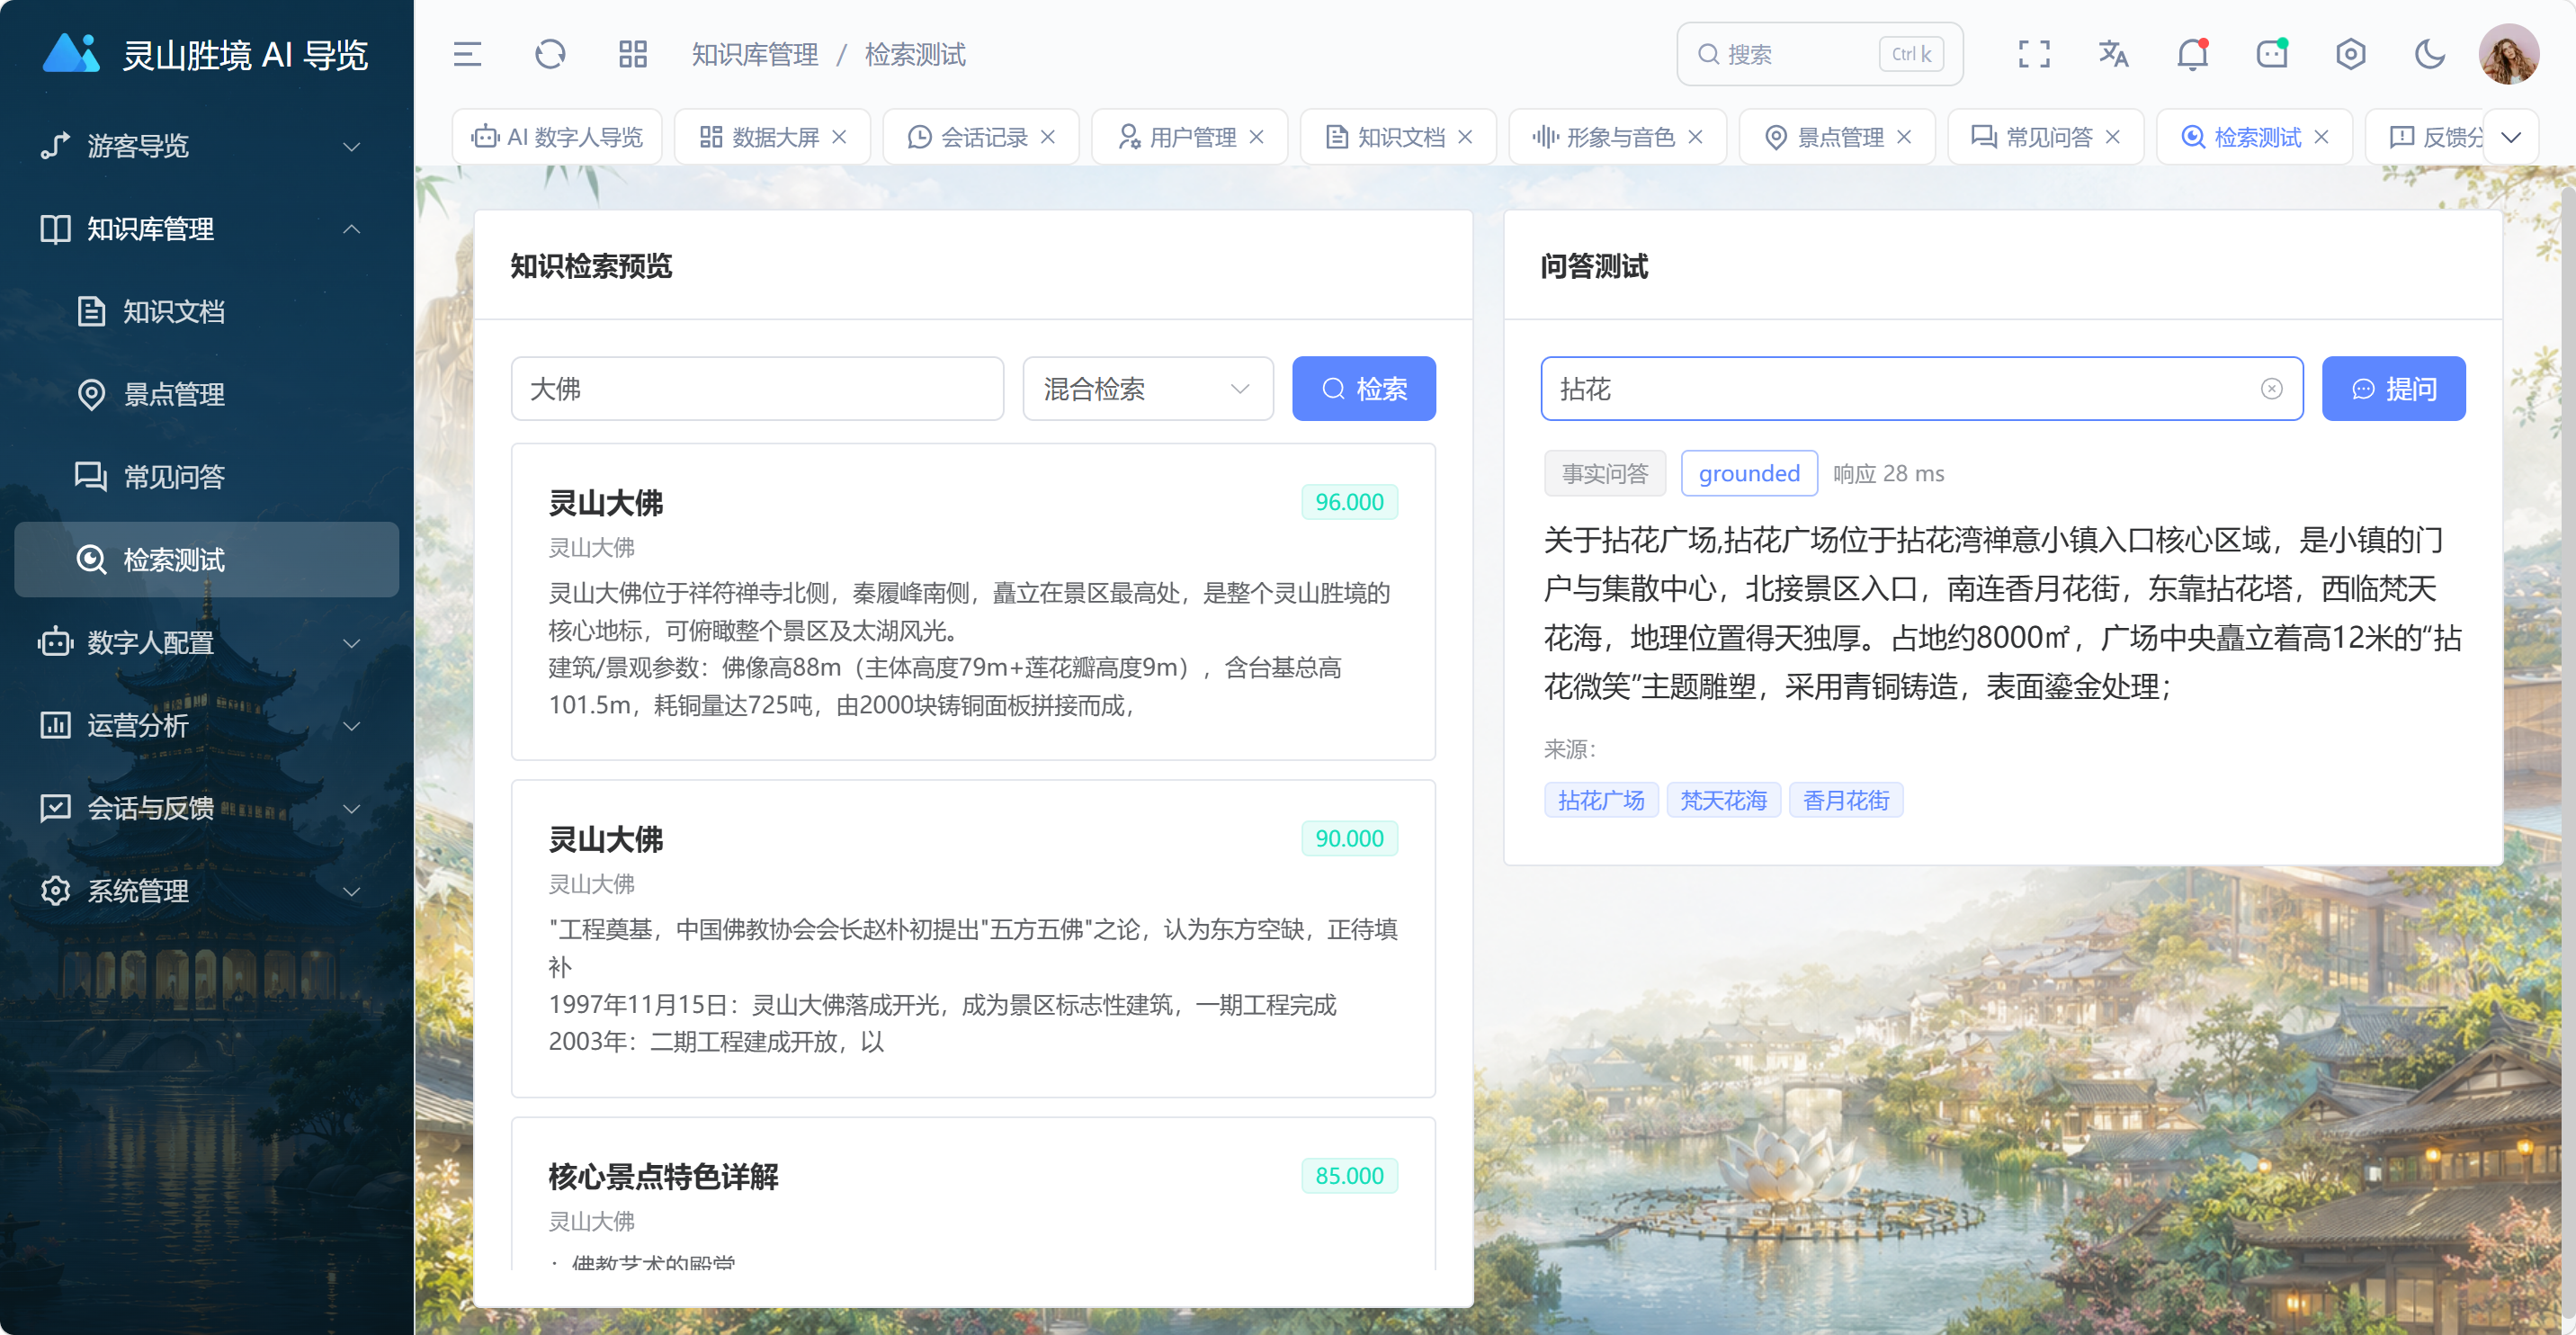
\includegraphics[width=0.95\textwidth]{figures/knowledge-console.png}%
  }{%
    \begin{tikzpicture}[x=1cm,y=1cm]
      \draw[rounded corners=5pt,very thick,guideTeal,fill=guideTealLight] (0,0) rectangle (14.2,6.6);
      \fill[guideTeal] (0,5.95) rectangle (14.2,6.6);
      \node[anchor=west,text=white,font=\bfseries] at (0.35,6.27) {知识库管理页面截图占位};
      \draw[rounded corners=3pt,fill=white,draw=guideTeal] (0.45,4.55) rectangle (4.20,5.55);
      \node at (2.33,5.05) {文档上传与状态};
      \draw[rounded corners=3pt,fill=white,draw=guideTeal] (4.45,4.55) rectangle (8.20,5.55);
      \node at (6.33,5.05) {知识分块统计与重建};
      \draw[rounded corners=3pt,fill=guideGoldLight,draw=guideGold] (8.45,4.55) rectangle (13.75,5.55);
      \node at (11.10,5.05) {混合检索测试与命中分数};
      \draw[rounded corners=3pt,fill=white,draw=guideTeal] (0.45,0.55) rectangle (8.20,4.20);
      \node[font=\bfseries] at (4.33,3.85) {文档与景点维护表};
      \foreach \y in {1.10,1.65,2.20,2.75,3.30}{\draw[guideGray!70] (0.85,\y) -- (7.80,\y);}
      \foreach \x in {2.15,4.15,6.15}{\draw[guideGray!50] (\x,0.90) -- (\x,3.55);}
      \draw[rounded corners=3pt,fill=white,draw=guideGold] (8.45,0.55) rectangle (13.75,4.20);
      \node[font=\bfseries] at (11.10,3.85) {检索结果预览};
      \draw[guideGold] (8.90,2.85) rectangle (13.30,3.40);
      \draw[guideGold] (8.90,1.95) rectangle (13.30,2.55);
      \draw[guideGold] (8.90,1.05) rectangle (13.30,1.65);
    \end{tikzpicture}%
  }
  \caption{知识库文档与检索管理页面图}\label{fig:knowledge-ui}
\end{figure}

\newpage
\section{业务数据与持久化}

SQLite实际建表覆盖管理员、游客会话、消息、反馈、景点、数字人配置、FAQ、知识文档、游客行为、路线选择和消息标注等业务对象。\textbf{事务型数据进入SQLite}；可从官方材料重建的\textbf{知识分块继续保存在JSON中}，从而避免将大段文本与高频会话写入混在同一数据路径。

\begin{table}[H]
  \centering
  \caption{SQLite业务表职责划分表}\label{tab:database}
  \begin{tabularx}{\textwidth}{p{0.25\textwidth}X p{0.25\textwidth}}
    \toprule
    表组 & 主要数据 & 生命周期与用途 \\
    \midrule
    admin\_users & 管理员、运营人员、角色和密码摘要 & 长期保存；管理端鉴权与权限控制 \\
    visitor\_sessions、messages、feedback & 会话、消息标签、时延、评分和文本反馈 & 持续积累；历史恢复与服务质量分析 \\
    scenic\_spots、admin\_faqs、knowledge\_documents & 景点覆盖、固定问答、上传文档状态 & 运营维护；影响问答和知识重建 \\
    digital\_human\_configs & 引擎、讯飞形象ID、Live2D模型ID、VCN、欢迎语、语速、情绪和服务状态 & 唯一启用配置下发游客端；支持云端与本地模型人工切换 \\
    tourist\_behavior、route\_selections & 线下消费行为和游客路线选择 & 运营分析；形成画像和路线偏好 \\
    message\_annotations & 正确、错误、需补知识等人工标注 & 质量闭环；生成知识补充草稿 \\
    \bottomrule
  \end{tabularx}
\end{table}

\section{接口规范}

后端以\filepath{/api}为\textbf{统一前缀}，OpenAPI合同记录\textbf{40条路径、45项操作}。成功响应采用\texttt{\{success,data,meta\}}，失败响应采用\texttt{\{success,error\}}；管理接口要求Bearer Token，游客接口使用匿名会话标识。请求日志记录方法、路径、状态码和耗时；长回答另提供SSE流式接口。接口命名遵循资源化路径，并将\textbf{检索证据、标签和阶段耗时}作为一等输出，便于前端展示与后台追踪。

\newpage
\section{部署拓扑}

生产模式下先构建Web产物，再由\textbf{Node.js同源提供静态资源、SPA回退和API}，减少跨域与多服务配置。数据库、知识库和Live2D模型位于本机数据或静态资源目录，讯飞数字人、大模型和语音能力通过HTTPS/WSS访问；讯飞形象流不可用时可由管理员启用\textbf{本地Live2D配置}，无密钥或其他云服务异常时，\filepath{DEMO_MODE}进入\textbf{本地确定性链路}。部署关系如图\ref{fig:deployment}所示。

\begin{figure}[H]
  \centering
  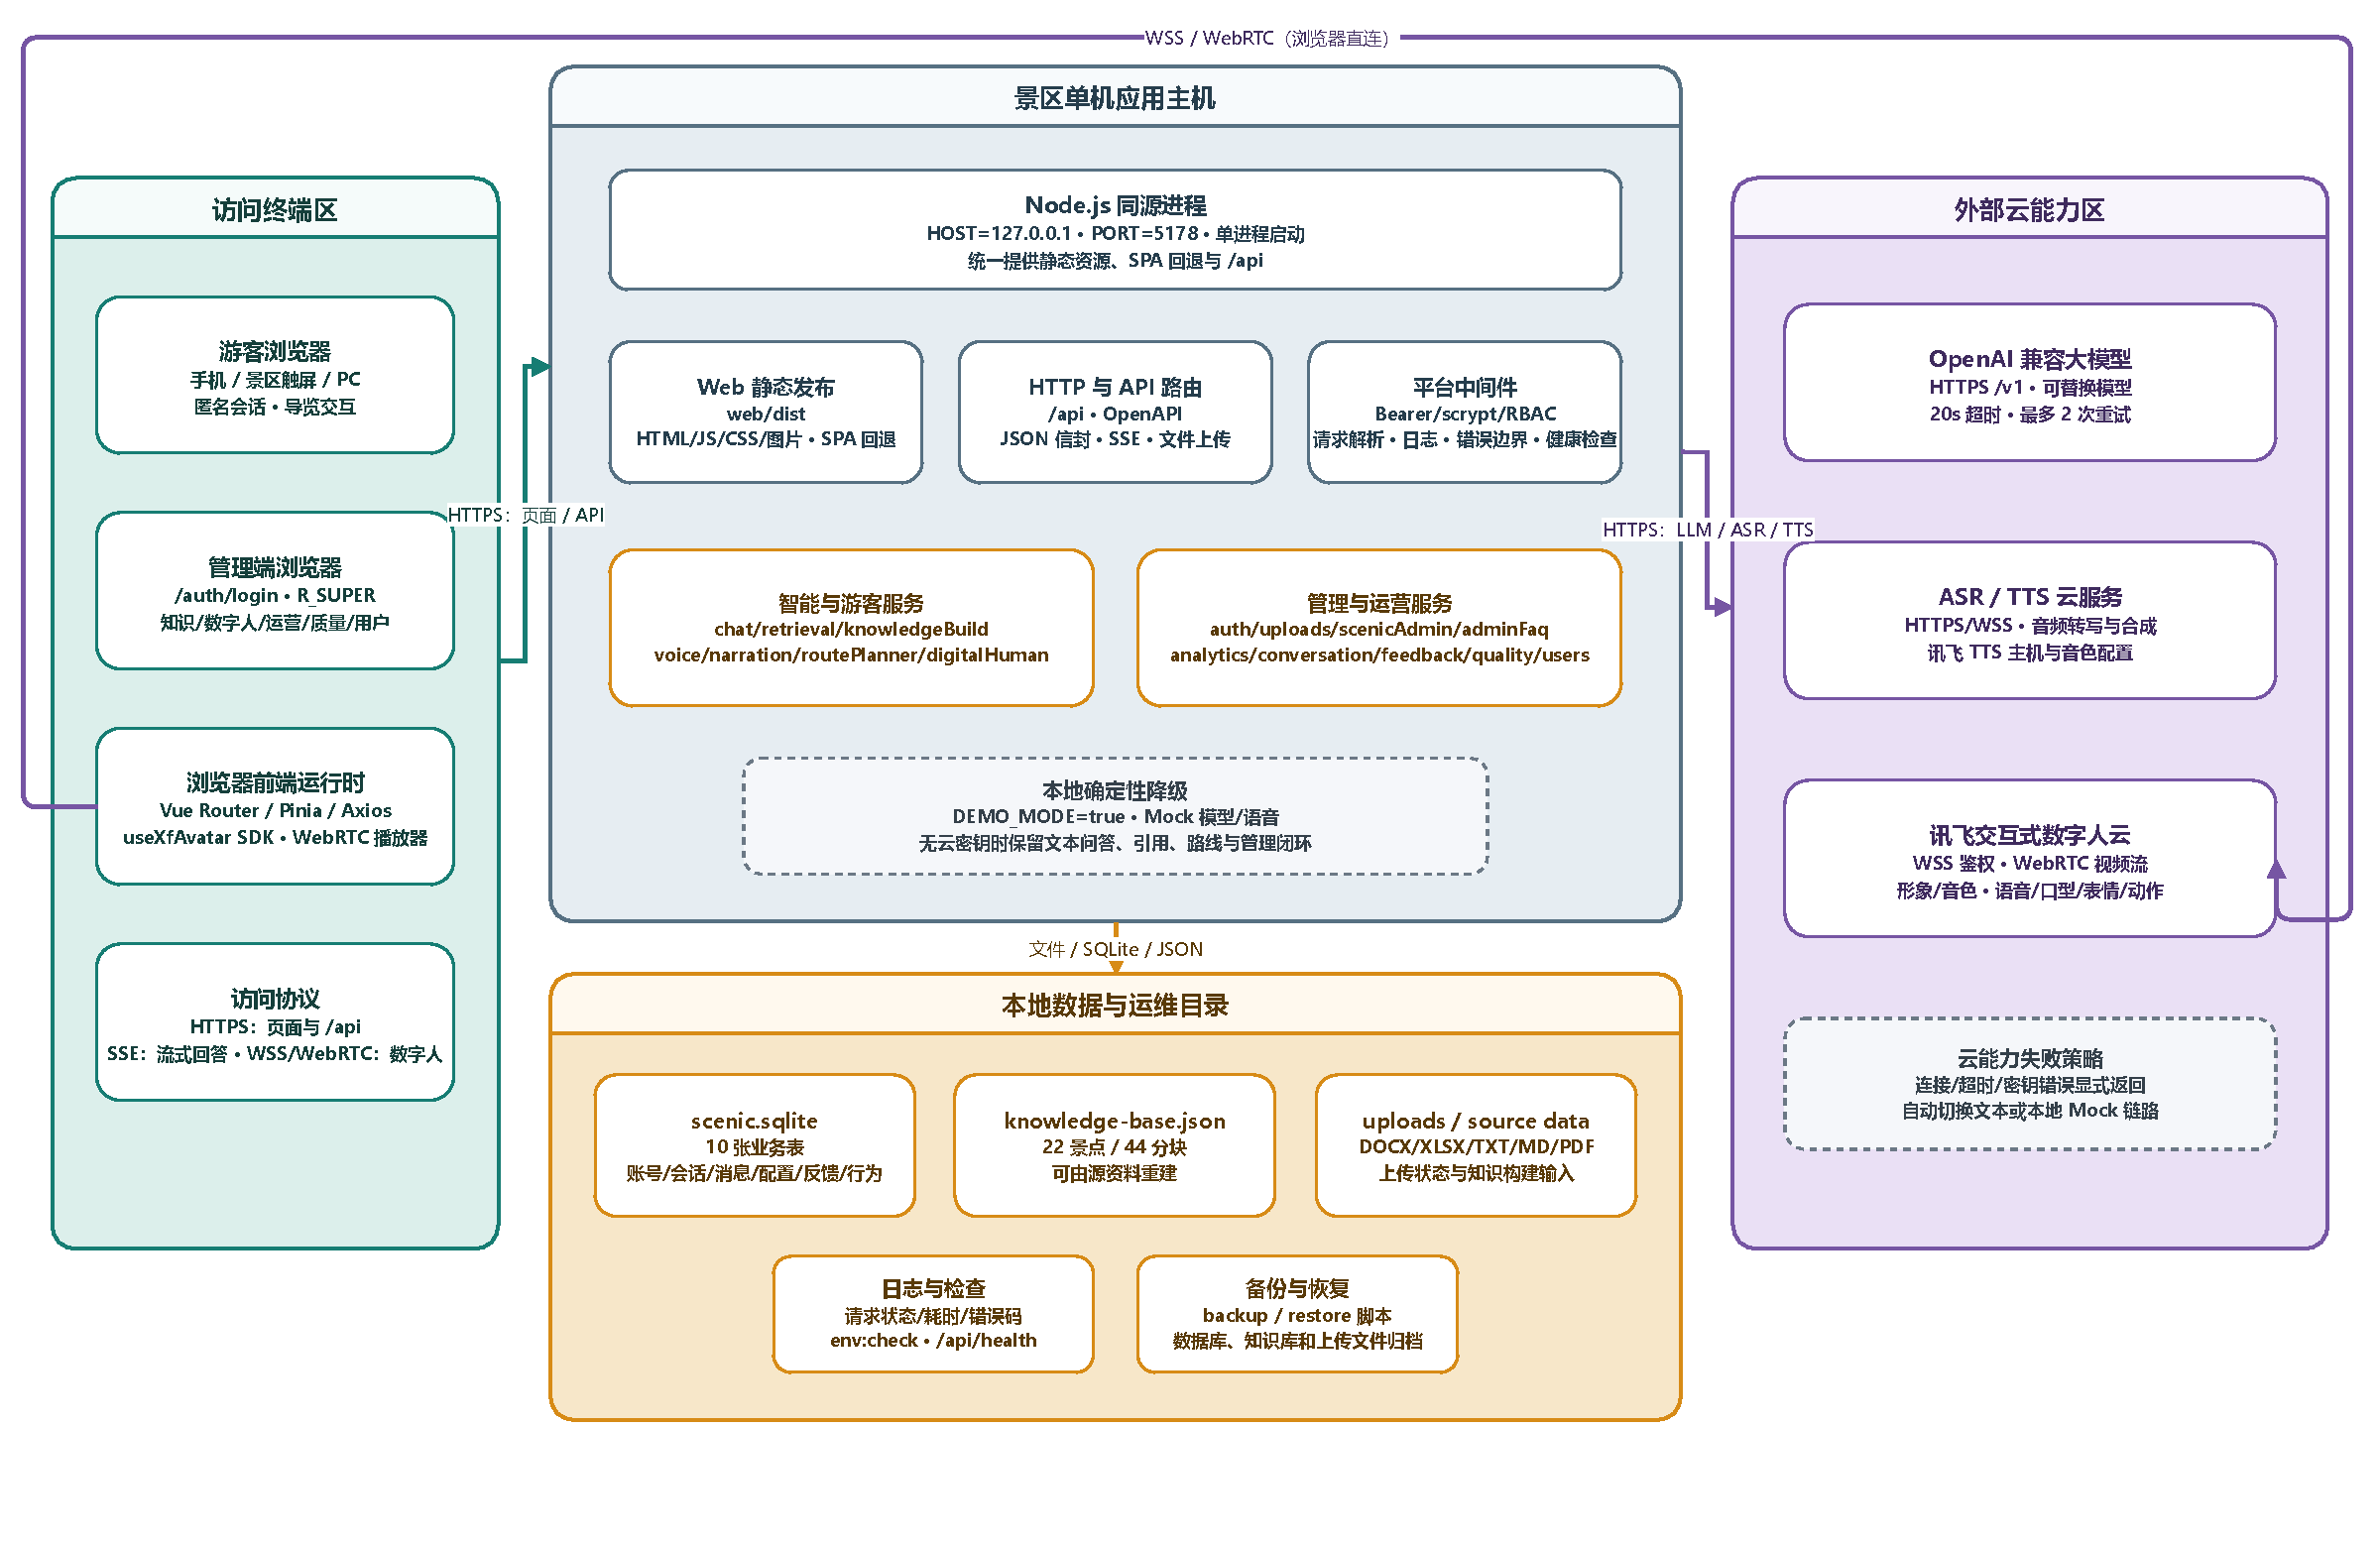
\includegraphics[width=0.98\textwidth]{deployment-topology.pdf}
  \caption{系统单机同源与云能力部署拓扑图}\label{fig:deployment}
\end{figure}

\textbf{配置项按职责拆分}：后端保存端口、模型提供者、数据库路径和演示模式；前端保存讯飞应用凭证、服务地址、形象与音色默认值，并随构建产物部署Live2D Cubism运行时及Haru、Hiyori、Kei、Hibiki四套模型。运行配置中的\filepath{engine}、\filepath{avatar_id}、\filepath{model_id}和\filepath{vcn}\textbf{决定游客端实际加载路径}。\textbf{密钥文件不纳入版本控制}，部署前使用\filepath{npm run env:check}检查Node版本、数据文件、目录、端口和云端凭证。

\newpage\chapter{质量、安全与可靠性设计}

\section{非功能指标}

赛题要求\textbf{事实问答准确率不低于90\%}、\textbf{语音问答时延合理}（示例阈值小于5秒）且系统稳定。设计上将指标拆分为可脚本验证的“准确、检索、构建、接口”与需真实浏览器和云账号验证的“口型、表情、云端时延”，避免以\textbf{离线Mock替代现场自然度结论}。

\begin{table}[H]
  \centering
  \caption{非功能指标与实现机制表}\label{tab:nfr}
  \begin{tabularx}{\textwidth}{p{0.16\textwidth}p{0.20\textwidth}X p{0.21\textwidth}}
    \toprule
    质量属性 & 目标 & 设计机制 & 验证方式 \\
    \midrule
    准确性 & 事实问答准确率$\geq90\%$ & 本地知识边界、混合检索、引用、无资料拒答 & 50题标准问答集 \\
    检索能力 & Top-3覆盖正确证据 & 实体、词项、意图、覆盖度加权与稳定重排 & 20条检索用例 \\
    响应性 & 语音链路目标$<5$秒 & FAQ缓存、分段TTS、阶段耗时、超时重试 & 现场云端实测与接口指标 \\
    稳定性 & 无崩溃、无长时间无响应 & 全局错误边界、请求日志、重复提交锁、演示降级 & 并发与降级脚本 \\
    可用性 & 移动端核心流程完整 & 五Tab信息架构、安全区、加载态、可恢复错误提示 & APK、小程序与HAP人工走查 \\
    跨平台性 & 同一业务覆盖Web、桌面和游客多端 & API合同复用，录音、定位、地图与WebView按端适配 & 各目标编译、包体校验与代表性设备运行 \\
    可维护性 & 内容和供应商可替换 & 服务模块、OpenAPI、知识重建、LLM/ASR/TTS适配器 & 工程检查与生产构建 \\
    \bottomrule
  \end{tabularx}
\end{table}

\section{安全与可信设计}

AI系统风险管理需要在治理、场景映射、测量和处置之间形成\textbf{持续闭环}\upcite{nist2023airmf}。本项目据此设置\textbf{四类控制}：输入侧敏感与越界检测，知识侧来源约束，生成侧引用和拒答，运营侧人工标注与知识修正。系统提示词明确\textbf{“仅基于灵山资料作答”}，不会用未检索到的模型记忆补全票价、开放时间等事实。

管理端使用\textbf{Bearer Token}\textbf{隔离游客权限}；密码采用\textbf{随机盐和scrypt派生摘要}。scrypt通过内存难解设计提高定制硬件暴力尝试的成本\upcite{percival2009scrypt}。云端凭证保存在环境变量，\textbf{不进入Git}；日志避免记录密钥原文，数据库备份与恢复脚本用于演示前保护数据状态。

\section{异常与降级策略}

\begin{table}[H]
  \centering
  \caption{关键风险与降级应对策略表}\label{tab:risk}
  \begin{tabularx}{\textwidth}{p{0.20\textwidth}p{0.18\textwidth}X p{0.20\textwidth}}
    \toprule
    风险事件 & 影响 & 系统应对 & 用户侧结果 \\
    \midrule
    讯飞形象凭证、额度或网络异常 & 云端视频流、口型或语音不可用 & 捕获SDK错误并释放实例；运营人员可启用\textbf{Live2D本地模型}，继续异常则切换文本/音频模式 & 角色切换过程可控，问答与路线仍可使用 \\
    大模型超时或密钥缺失 & 无法生成自然语言答案 & 超时重试；演示模式调用\textbf{本地确定性提供者} & 获得稳定的有据答案 \\
    ASR不可用或浏览器不支持 & 无法完成语音输入 & 显示文字输入，并支持模拟转写演示 & 用户可继续文本提问 \\
    TTS长文本或失败 & 首次播放慢、播报中断 & 断句分段合成，先返回可播放片段 & 答案文本立即可读 \\
    腾讯地图离线、Key或SDK异常 & 在线底图无法加载 & Web恢复Leaflet/手绘层；游客端保留原生地图与本地手绘图切换 & 点位、路线、搜索和讲解仍可使用 \\
    定位权限拒绝或GPS漂移 & 无法自动居中或最近点判断偏差 & 保留当前中心、搜索与手动选点；最近点只作为建议 & 游客可手工选择景点继续导览 \\
    移动端WebView或平台能力受限 & 云数字人或在线地图在特定端不可用 & 微信使用本地数字人表现；HarmonyOS等端保留手绘地图和TTS & 核心问答、地图点位与路线不中断 \\
    知识库未构建或低相关 & 可能无证据或产生幻觉 & 返回未构建状态；低相关问题进入\textbf{诚实拒答} & 不编造景区事实 \\
    数据库或演示数据损坏 & 历史、配置和后台不可用 & 备份恢复；必要时重建演示数据库 & 可恢复到预置状态 \\
    \bottomrule
  \end{tabularx}
\end{table}

\section{可观测与运维}

每次HTTP请求记录方法、路径、状态与耗时；问答响应额外记录\textbf{检索和LLM耗时}，语音响应记录ASR、RAG、LLM、TTS及总耗时。管理员可从会话详情查看\textbf{答案标签、情绪、时延与反馈}，并对错误消息标注“错误”或“需补知识”。\filepath{env:check}、\filepath{backup}、\filepath{restore}、\filepath{test:concurrency}和\filepath{test:demo-mode}脚本共同覆盖\textbf{部署前检查、数据保护和现场演示保障}。桌面交付另执行Web构建、ASAR树、\filepath{node:sqlite}运行时、系统架构和安装包后缀校验；移动交付记录AppID、包标识、权限声明、版本号和产物路径。

\section{隐私与数据最小化}

游客侧以\textbf{匿名会话标识}工作，不要求采集身份证、手机号等身份数据；定位只在游客主动点击定位后请求，录音只在按下录音按钮并授予麦克风权限后上传，地图与语音服务不把原始坐标、音频或云端凭证写入前端持久化配置。运营大屏处理年龄段、性别、消费和满意度等统计字段，\textbf{输出聚合趋势而非个人画像明细}。正式落地时应增加明确告知、保存期限、日志脱敏、角色最小权限和备份加密策略，并为语音上传与云端数字人处理提供\textbf{用户授权入口}。

\newpage\chapter{测试评估与应用价值}

\section{测试策略与结果}

测试遵循\textbf{“知识数据--服务函数--接口场景--工程构建”四层结构}。2026年7月16日在当前工程执行后端完整性、数据库、问答、检索、路线、语音、数字人、分析、质量、并发和降级脚本，\textbf{全部通过}；前端TypeScript检查验证五语言消息元组和数字人配置类型，Vite生产构建通过，共转换\textbf{2838个模块}。

\begin{table}[H]
  \centering
  \caption{项目自动化测试与评估结果汇总表}\label{tab:test-results}
  \begin{tabularx}{\textwidth}{p{0.25\textwidth}p{0.20\textwidth}X p{0.14\textwidth}}
    \toprule
    验证项 & 数据规模或场景 & 当前结果 & 结论 \\
    \midrule
    工程完整性检查 & 目录、数据、合同、配置 & \filepath{check}通过 & 通过 \\
    SQLite数据库测试 & 预置、登录、会话、FAQ、景点、数字人等8项 & 8/8通过 & 通过 \\
    问答场景测试 & 事实、讲解、路线、越界、敏感、多轮、缓存等 & 13/13通过 & 通过 \\
    标准问答评估 & 50题；48条可回答、2条拒答 & 50/50，准确率100\% & 超过90\%阈值 \\
    检索评估 & 20条用例 & Top-1标题95\%；Top-3标题/景点/词项100\% & 通过 \\
    五语言国际化 & 五元组业务词典、框架覆盖、Locale枚举与生产构建 & TypeScript检查与五语言资源构建成功 & 通过 \\
    业务模块测试 & 路线、语音、数字人配置、分析、服务质量 & 全部通过 & 通过 \\
    稳定性测试 & 并发问答与演示降级 & 全部通过 & 通过 \\
    前端生产构建 & Vue类型检查与Vite构建 & 2838模块转换，构建成功 & 通过 \\
    \bottomrule
  \end{tabularx}
\end{table}

需要说明：50题问答评估使用项目内置\textbf{确定性Mock模型}，验证的是知识命中、场景分类、引用和答案要点，\textbf{不等同于真实云模型的自然度评价}；数字人实时画面、口型自然度和云端语音总时延须在有讯飞额度、外网和真实浏览器的演示环境人工验证。

\begin{figure}[H]
  \centering
  \begin{tikzpicture}[x=1.10cm,y=0.82cm]
    \draw[->,thick,guideGray] (0,0) -- (10.2,0) node[right,font=\small] {准确率/召回率};
    \foreach \x/\lab in {0/0,2/20,4/40,6/60,8/80,10/100}{
      \draw[guideGray] (\x,0.08) -- (\x,-0.08) node[below,font=\scriptsize] {\lab\%};
    }
    \fill[guideTeal] (0,0.55) rectangle (9.5,1.05);
    \node[anchor=east,font=\small] at (-0.15,0.80) {检索Top-1};
    \node[anchor=west,font=\small\bfseries] at (9.55,0.80) {95\%};
    \fill[guideTeal] (0,1.45) rectangle (10,1.95);
    \node[anchor=east,font=\small] at (-0.15,1.70) {检索Top-3};
    \node[anchor=west,font=\small\bfseries] at (10.05,1.70) {100\%};
    \fill[guideGold] (0,2.35) rectangle (10,2.85);
    \node[anchor=east,font=\small] at (-0.15,2.60) {标准问答};
    \node[anchor=west,font=\small\bfseries] at (10.05,2.60) {100\%};
    \draw[dashed,very thick,red!65!black] (9,0.25) -- (9,3.15);
    \node[anchor=south,font=\scriptsize,text=red!65!black] at (9,3.15) {赛题阈值：90\%};
  \end{tikzpicture}
  \caption{核心问答与检索指标对比图}\label{fig:evaluation}
\end{figure}

\section{行业应用价值}

对于游客，产品降低导览服务获取门槛，\textbf{五语言界面}支持不同语言游客理解导览操作，个性路线和可见引用提升自由探索能力与信任；对于景区，产品将重复讲解、FAQ维护、游客反馈和运营分析集中到\textbf{统一平台}，缓解旺季人员压力；对于文旅内容运营方，景点实体、知识分块、云端/本地数字人形象、音色和路线模板\textbf{均可配置}，具备迁移到其他景区的基础。

在真实部署中，可按照\textbf{“单景区知识库验证--多终端接入--运营数据闭环--多景区复制”}的路径渐进推广。下一阶段可增加GPS到点讲解、向量检索、多语种景点知识内容与人工术语审校、弱网缓存及票务/客流系统对接，但这些扩展不影响当前\textbf{五语言界面与赛题功能闭环}。

\newpage\chapter{创新实践}

本项目的创新不是孤立叠加大模型、语音或数字人，而是围绕景区导览的真实约束，把“可信知识、自然表达、个性路线、运营数据和稳定交付”组织成\textbf{可运行、可验证的连续链路}。每项创新均有对应的数据结构、服务模块、界面状态或测试脚本支撑，能够在比赛演示中说明\textbf{输入、处理、输出与异常路径}。

\section{可信智能与沉浸表达创新}

\subsection{从相似命中升级为有边界的证据链}

通用问答容易把模型记忆与景区事实混合，项目因此将景点实体、别名、意图、关键词和查询覆盖度纳入同一\textbf{混合评分}，并在生成前执行敏感、越界、低相关和资料缺失判断。返回结构不只包含答案，还包含文档、章节、景点、质量标签及阶段耗时。游客可以知道“答案从哪里来”，管理员也能定位“问题在哪一步发生”，使RAG从后台检索组件转化为\textbf{可感知的信任机制}。

\subsection{从局部翻译升级为全业务五语言一致性}

系统将框架导航与景区业务文案拆分维护、统一合并，业务键使用\textbf{固定五语言元组}，使新页面在类型检查阶段即可发现译文数量不完整。语言状态同时驱动菜单、面包屑、标签页、表单、状态提示和浏览器语音Locale，并持久化到用户配置。该设计把国际化从外层布局装饰转化为\textbf{贯穿导览与运营流程的基础能力}，同时明确\textbf{不对景点知识和历史内容进行未经审校的自动翻译}。

\subsection{从单一云端形象升级为配置驱动的双引擎表达}

问答服务统一输出事实性、场景、质量和情绪标签，数字人模块再映射为倾听、思考、讲解、微笑、致歉和引导等状态，同时控制TTS情绪、口型、表情与动作。\textbf{统一调度器}可装载讯飞云端流式形象或本地Live2D模型，两套引擎\textbf{共享播报、音频解锁和打断契约}；管理端通过形象、音色目录及启用配置决定实际角色。该设计既避免前端仅凭关键词随机触发动作，也在保持角色切换可控的前提下提供本地模型冗余，形成\textbf{“语义决策—引擎选择—表达执行—状态回传”闭环}。

\subsection{从路线清单升级为可继续对话的讲解服务}

路线推荐将时长、兴趣、同行群体、体力与景点图统一为\textbf{可解释评分}，得到主路线后继续执行压缩、避阶和冲突偏好折中。每个节点不仅展示顺序与推荐理由，还可直接转交数字人发起景点讲解，游客能够沿着“规划路线—到达节点—继续追问—获得讲解”自然推进。路线因此不再是静态结果页，而成为\textbf{贯穿游览过程的对话入口}。

\newpage
\section{运营闭环与工程落地创新}

\subsection{线上会话与线下行为的双数据观察}

管理端同时汇聚问题、引用、情绪、评分、响应耗时等线上会话数据，以及\textbf{522条灵山相关消费行为记录}。数据大屏据此展示热门问答、景点关注度、情感分布、消费结构和人群特征，使\textbf{“游客问了什么”与“游客如何游览和消费”相互印证}，为知识补充、路线调整和服务资源配置提供依据。

\subsection{从低满意会话回流到知识修正}

运营人员可以从低评分或异常会话进入消息标注，将记录归类为回答正确、回答错误、资料缺失或表达不佳；其中\textbf{资料缺失项可生成知识补充草稿}，经人工核验后进入知识重建或FAQ高优先级通道。修订后的内容再通过检索测试和标准问答集验证，构成\textbf{“发现问题—人工判断—补充知识—重新评估”的质量实践}。

\subsection{面向比赛现场的确定性降级链路}

项目把讯飞数字人、Live2D模型、云端TTS、云端ASR和大模型分别视为\textbf{可替换能力}。讯飞形象流不可用时，运营人员可切换本地Live2D配置；任一语音或模型服务继续不可用时，系统\textbf{优先保留已有文本答案、引用、本地检索和路线推荐}，并通过\filepath{DEMO_MODE}提供确定性链路。该机制不是隐藏错误，而是\textbf{明确显示引擎、降级阶段和原因}，使核心业务叙事不因网络、额度或设备差异而中断。

\begin{table}[H]
  \centering
  \small
  \renewcommand{\arraystretch}{1.05}
  \caption{创新实践与工程证据对应表}\label{tab:innovation-evidence}
  \begin{tabularx}{\textwidth}{p{0.23\textwidth}X p{0.27\textwidth}}
    \toprule
    创新实践 & 工程落点 & 可验证证据 \\
    \midrule
    有界RAG证据链 & 混合评分、护栏、重排、引用与质量标签 & 检索测试、答案来源和响应耗时 \\
    五语言全局一致性 & 基础词典、框架覆盖、业务五元组、语言持久化 & 全局切换、五语言页面与生产构建 \\
    双引擎状态数字人 & 回答标签、统一调度器、讯飞SDK、Live2D与音色目录 & 云端/本地形象、口型状态、配置切换和打断操作 \\
    路线讲解一体化 & 偏好评分、路线自适应、节点讲解入口 & 推荐理由、备选路线与节点追问 \\
    双数据运营观察 & 会话反馈与线下行为统一分析 & KPI、热度、情绪、画像和消费结构 \\
    知识质量修正闭环 & 消息标注、知识草稿、FAQ与重建流程 & 低满意会话复盘及检索回归测试 \\
    确定性降级交付 & 云能力适配器、错误状态和\filepath{DEMO_MODE} & 断网、无密钥和数字人失败场景 \\
    \bottomrule
  \end{tabularx}
\end{table}

\newpage\chapter{总结与展望}

\section{项目总结}

数智游踪已围绕A5“景区导览服务AI数字人”赛题形成\textbf{完整产品闭环}：游客端以数字人为统一入口，支持文本与语音问答、景点讲解、个性路线与满意度反馈；管理端覆盖身份权限、知识维护、数字人配置、会话质量与运营大屏。系统完成简体中文、英文、韩文、繁体中文和日文的\textbf{全局界面国际化}，并以讯飞云端流式数字人与Live2D本地模型形成\textbf{配置驱动的双引擎体系}；底层以本地知识和引用约束事实边界，并通过SQLite、OpenAPI、自动化测试与单机同源部署保证\textbf{工程可复现性}。

项目价值不依赖单一模型能力，而来自“资料入库—熟悉语言操作—有据回答—数字人表达—数据沉淀—知识修正”的\textbf{持续循环}。50条标准问答、20条检索用例、数字人配置测试与五语言生产构建共同证明，当前实现既可支撑比赛演示，也具备进入\textbf{单景区试运行}的基础。

\section{后续展望}

后续建设坚持\textbf{先验证价值、再扩大范围}：近期接入GPS或蓝牙信标实现到点触发与弱网缓存，并补充\textbf{经人工审校的多语种景点资料}；中期对接票务、客流与活动排期系统，使路线推荐兼顾\textbf{实时拥挤度与运营目标}；规模化阶段进一步将景点实体、语言包、数字人形象与指标看板抽象为\textbf{景区级配置}，形成\textbf{可复制的多租户能力}，并持续校准模型与交互策略。

\section{最后的话}

感谢指导老师\textbf{陈子淮}在选题方向、系统设计与文档打磨过程中的悉心指导；感谢第十五届“中国软件杯”大赛\textbf{组委会}搭建的竞赛与交流平台，让团队得以在真实赛题中锤炼产品与技术；也感谢\textbf{数智游踪队}三位队友的通力协作，从知识库、算法到前端与数字人各司其职、彼此补位，共同完成了这份作品。


\newpage
\printbibliography[heading=bibintoc,title=参考文献]

\end{document}
